% !TeX root = ./main.tex

\chapter{正问题的数值实验}

本章使用了四个数值实验来测试 cPINNs 算法的可行性。同时,本章利用第一个数值实验对网络结构的不同配置进行了一些探索,为接下来的实验设置提供参考;第二个数值实验中物理方程带有参数项 $\kappa$ ,以测试算法对不同参数物理方程模型的求解能力;后两个数值实验分别为稳态形式的耦合模型以及交界面为 BJS 形式的耦合模型正问题实验,本算法只需对损失函数中的时间项以及初值条件项进行轻微改动便可对两者进行迁移,进一步验证了 cPINNs 算法的通用性。

\section{实验一:真解数值实验}

本节使用一个具有解析解的数值算例进行网络结构探索实验。其中 $\Of = (0, 1) \times (1, 2), \Op =  (0, 1) \times (0, 1), T = (0,1), \iB = (0, 1) \times \{1\}, \vec{n} = \overrightarrow{(0, -1)}^T, \vec{\tau} = \overrightarrow{(0, 1)}^T$;对应的解析解由公式 \ref{eq:example1} 给出;算例的物理方程参数为:$ \rho = \mu = S_0 = g = \kappa = \alpha = 1, \matfmt{K} = \frac{\rho g \kappa \matfmt{I} }{\mu} = \matfmt{I}$,另外 Navier-Stokes 方程的加速度场函数与 Darcy 方程组中的源项 $\gf, \fp$ 可由解析解计算导出。容易验证其满足 ~\eqref{eq:NS},~\eqref{eq:Darcy} 与 ~\eqref{eq:Interface} 条件:

\begin{equation}\label{eq:example1}
    \left\{
    \begin{aligned}
        \Ufi[1]^* &= (x^2 \* (y-1)^2 + y) \* \frac{cos(t)}{3} &\textrm{ in } \Df\\
        \Ufi[2]^* &= (-\frac{2}{3} \* x \* (y-1)^3 + 2 - \pi \* sin(\pi \* x)) \frac{cos(t)}{3} &\textrm{ in } \Df\\
        \pf^* &= (2 - \pi \* sin(\pi \* x)) \* sin(\pi \* \frac{y}{2}) \* \frac{cos(t)}{3} &\textrm{ in } \Df\\
        \Upi[1]^* &= \pi^2 \* (-y - cos(\pi \* y) + 1) \* \frac{cos(t)}{3} \* cos(\pi \* x) &\textrm{ in } \Dp\\
        \Upi[2]^* &= \left(\pi \* sin(\pi \* x) - 2\right) \* \left(\pi \* sin(\pi \* y) - 1 \right) \* \frac{cos(t)}{3} &\textrm{ in } \Dp\\
        \pp^* &= (2 - \pi \* sin(\pi \* x)) \* (1 - y - cos(\pi \* y)) \* \frac{cos(t)}{3} &\textrm{ in } \Dp
    \end{aligned}
    \right.
\end{equation}

\newcommand{\slf}{\mathrm{logistic}}
\newcommand{\htf}{\tanh}
\newcommand{\relu}{\mathrm{ReLU}}

网络结构采用如下设置:$\NN_f, \NN_p$ 均采用全连接神经网络,各隐藏层网络的神经元个数均为 $32$,激活函数将分别测试标准逻辑斯谛函数(Standard Logistic Function) $\slf (x) = (1 + e^{-x})^{-1}$,双曲正切函数(Hyperbolic Tangent Function) $\htf (x) = \frac{e^x - e^{-x}}{e^x + e^{-x}}$ 以及工程上常用的整流线性单位函数(Rectified Linear Unit, ReLU) $\relu (x)= \max(0,x)$;网络的隐藏层数分别使用 $1,2,4,6,8$ 进行测试。

\newcommand{\num}[2]{{#1} \times 10^{#2}}
训练策略上,容许误差 $\varepsilon = \num{1}{-10}$,训练阈值参数 $n_T = 30$;初始学习率设置为 $\num{1}{-3}$,自适应调整策略中学习率调整误差阈值 $\epsilon_{lr} = \num{1}{-8}$,学习率调整耐心阈值 $n_{lr} = 10$,学习率调整衰减率 $r_{lr} = 0.5$,采取Adam参数更新策略。神经网络参数的初始化方法采用 Kaiming 初始化。

各训练集数据的采集策略为:对耦合模型的各区域 $\Df,\BDf,\IDf,\Dp,\BDp,\IDp,\iBD$ 进行均匀随机采样生成对应训练集,采样的数据点比例为 $50:4:1:50:4:1:5$,共采集 $3 \times {10}^{5}$ 个样本数据点。

表 展示了不同的网络结构配置下的实验结果,其中相对误差由 ~\eqref{eq:relative_error} 定义,注意其数值计算类似于损失函数同样是按照均匀采样离散化后再计算的。

\newcommand{\relaErr}{\mathrm{error}^{rel}}
\newcommand{\toRelaErr}[2]{
    \frac{\sqrt{\|{#1}^{\NN} - {#1}^* \|_{\Lp[2]}^2 + \|{#2}^{\NN} - {#2}^* \|_{\Lp[2]}^2}}{\sqrt{\|{#1}^* \|_{\Lp[2]}^2 + \|{#2}^* \|_{\Lp[2]}^2}}
}
\begin{equation}\label{eq:relative_error}
    \begin{aligned}
        \relaErr_{u} = \toRelaErr{\Uf}{\Up} \\
        \relaErr_{p} = \toRelaErr{\pf}{\pp}
    \end{aligned}
\end{equation}


\begin{table}[H]
    \centering
    \caption{实验一结果}
    \begin{tabular}{cccc}
        \toprule
        网络层数 & 激活函数 & $\relaErr_{u}$ & $\relaErr_{p}$ \\
        \midrule
        1  & $\relu$ & $\num{7.2315}{1}$ & $\num{1.0311}{2}$ \\
        1  & $\slf $ & $\num{5.5137}{1}$ & $\num{9.2287}{1}$ \\
        1  & $\htf $ & $\num{5.4759}{1}$ & $\num{9.0141}{1}$ \\
        2  & $\relu$ & $\num{6.2912}{-1}$ & $\num{2.9390}{0}$ \\
        2  & $\slf $ & $\num{3.3533}{-1}$ & $\num{8.3449}{-1}$ \\
        2  & $\htf $ & $\num{2.3089}{-1}$ & $\num{6.1142}{-1}$ \\
        4  & $\relu$ & $\num{5.7582}{-1}$ & $\num{1.2959}{0}$ \\
        4  & $\slf $ & $\num{2.8264}{-2}$ & $\num{1.0619}{-1}$ \\
        4  & $\htf $ & $\num{2.7503}{-2}$ & $\num{9.8046}{-2}$ \\
        6  & $\relu$ & $\num{4.9802}{-1}$ & $\num{7.4808}{-1}$ \\
        6  & $\slf $ & $\num{3.0148}{-2}$ & $\num{1.0793}{-1}$ \\
        6  & $\htf $ & $\num{2.7495}{-2}$ & $\num{1.0071}{-1}$ \\
        8  & $\relu$ & $\num{5.1132}{-1}$ & $\num{9.7828}{-1}$ \\
        8  & $\slf $ & $\num{2.7799}{-2}$ & $\num{9.9716}{-2}$ \\
        8  & $\htf $ & $\num{2.6945}{-2}$ & $\num{9.6993}{-2}$ \\
        \bottomrule
    \end{tabular}
    \label{tab:example1}
\end{table}

由此可推测当每层神经元数量有限时,若网络层数太少,由于参数量不够会导致拟合不成功;另一方面拟合效果不会随着层数的增加而无限制提高下去。虽然激活函数 $\relu$ 在深度学习实践中很常见,但在此问题中效果不如 $\slf$ 与 $\htf$;$\slf, \htf$ 的拟合效果接近,但是在实验中观察到使用 $\htf$ 时训练网络的收敛速度快于 $\slf$,如图 \ref{fig:example1_loss}所示,推测是前者的梯度更加陡峭所致。

\begin{figure}[H]
    \centering
    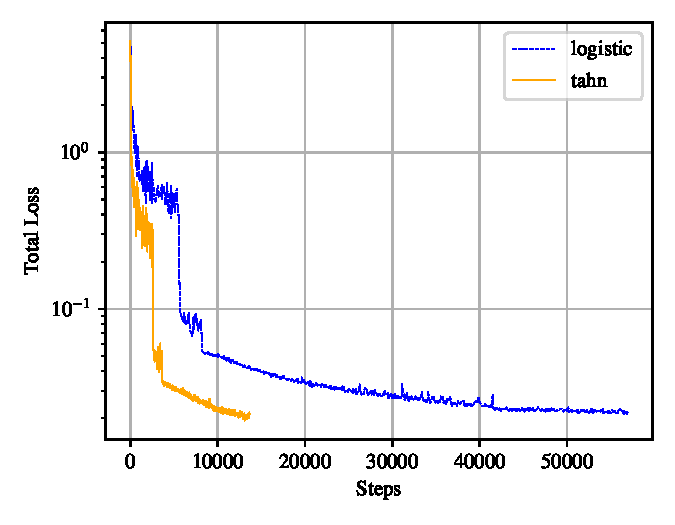
\includegraphics[width=0.4\linewidth]{images/example1_loss.pdf}
    % \caption*{}
    \caption{$\slf$ 与 $\htf$ 实验效果的比较}
    \label{fig:example1_loss}
\end{figure}

以网络隐藏层数设为4,激活函数选为 $\htf$ 时的拟合实验为例,此时网络已经基本能够拟合出真解,数值真解与网络拟合结果对比如图 \ref{fig:example1_exact}, \ref{fig:example1_fitted} 所示。此时再增加网络层数,最终的拟合效果提升有限,出于平衡拟合效果与网络计算量的考虑,选取这一配置作为接下来的实验配置。

\begin{figure}[H]
    \centering
    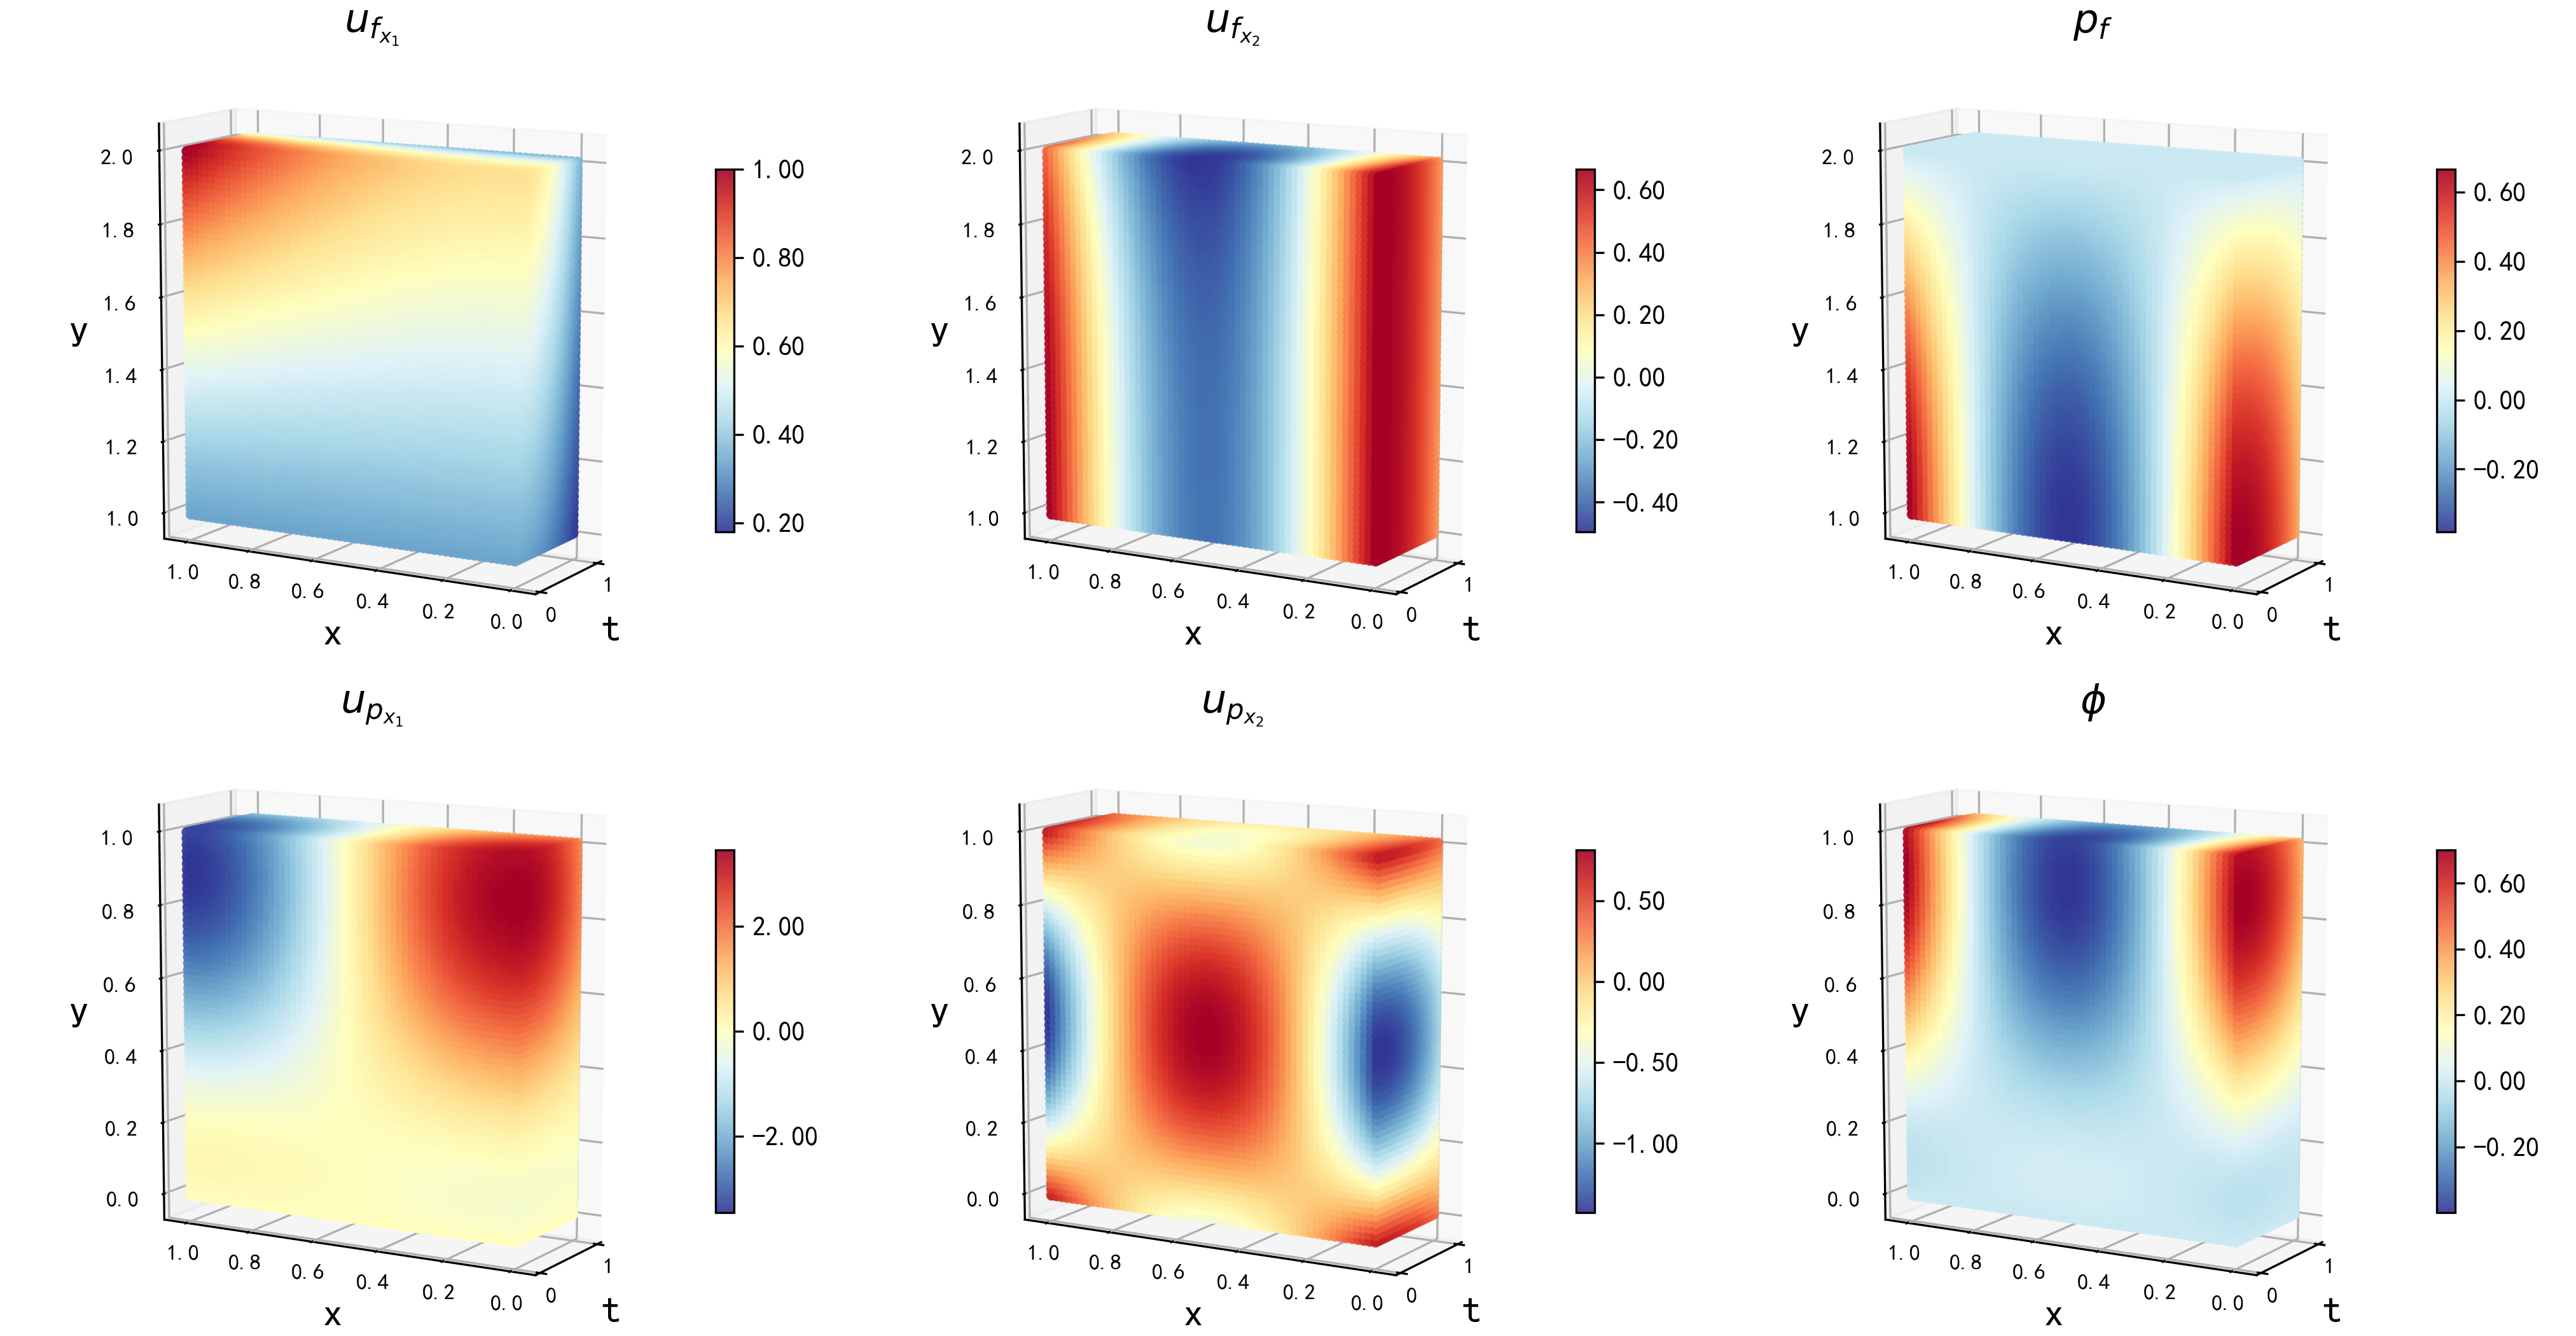
\includegraphics[width=0.75\linewidth]{images/example1_exact.png}
    % \caption*{}
    \caption{实验一的数值真解}
    \label{fig:example1_exact}
    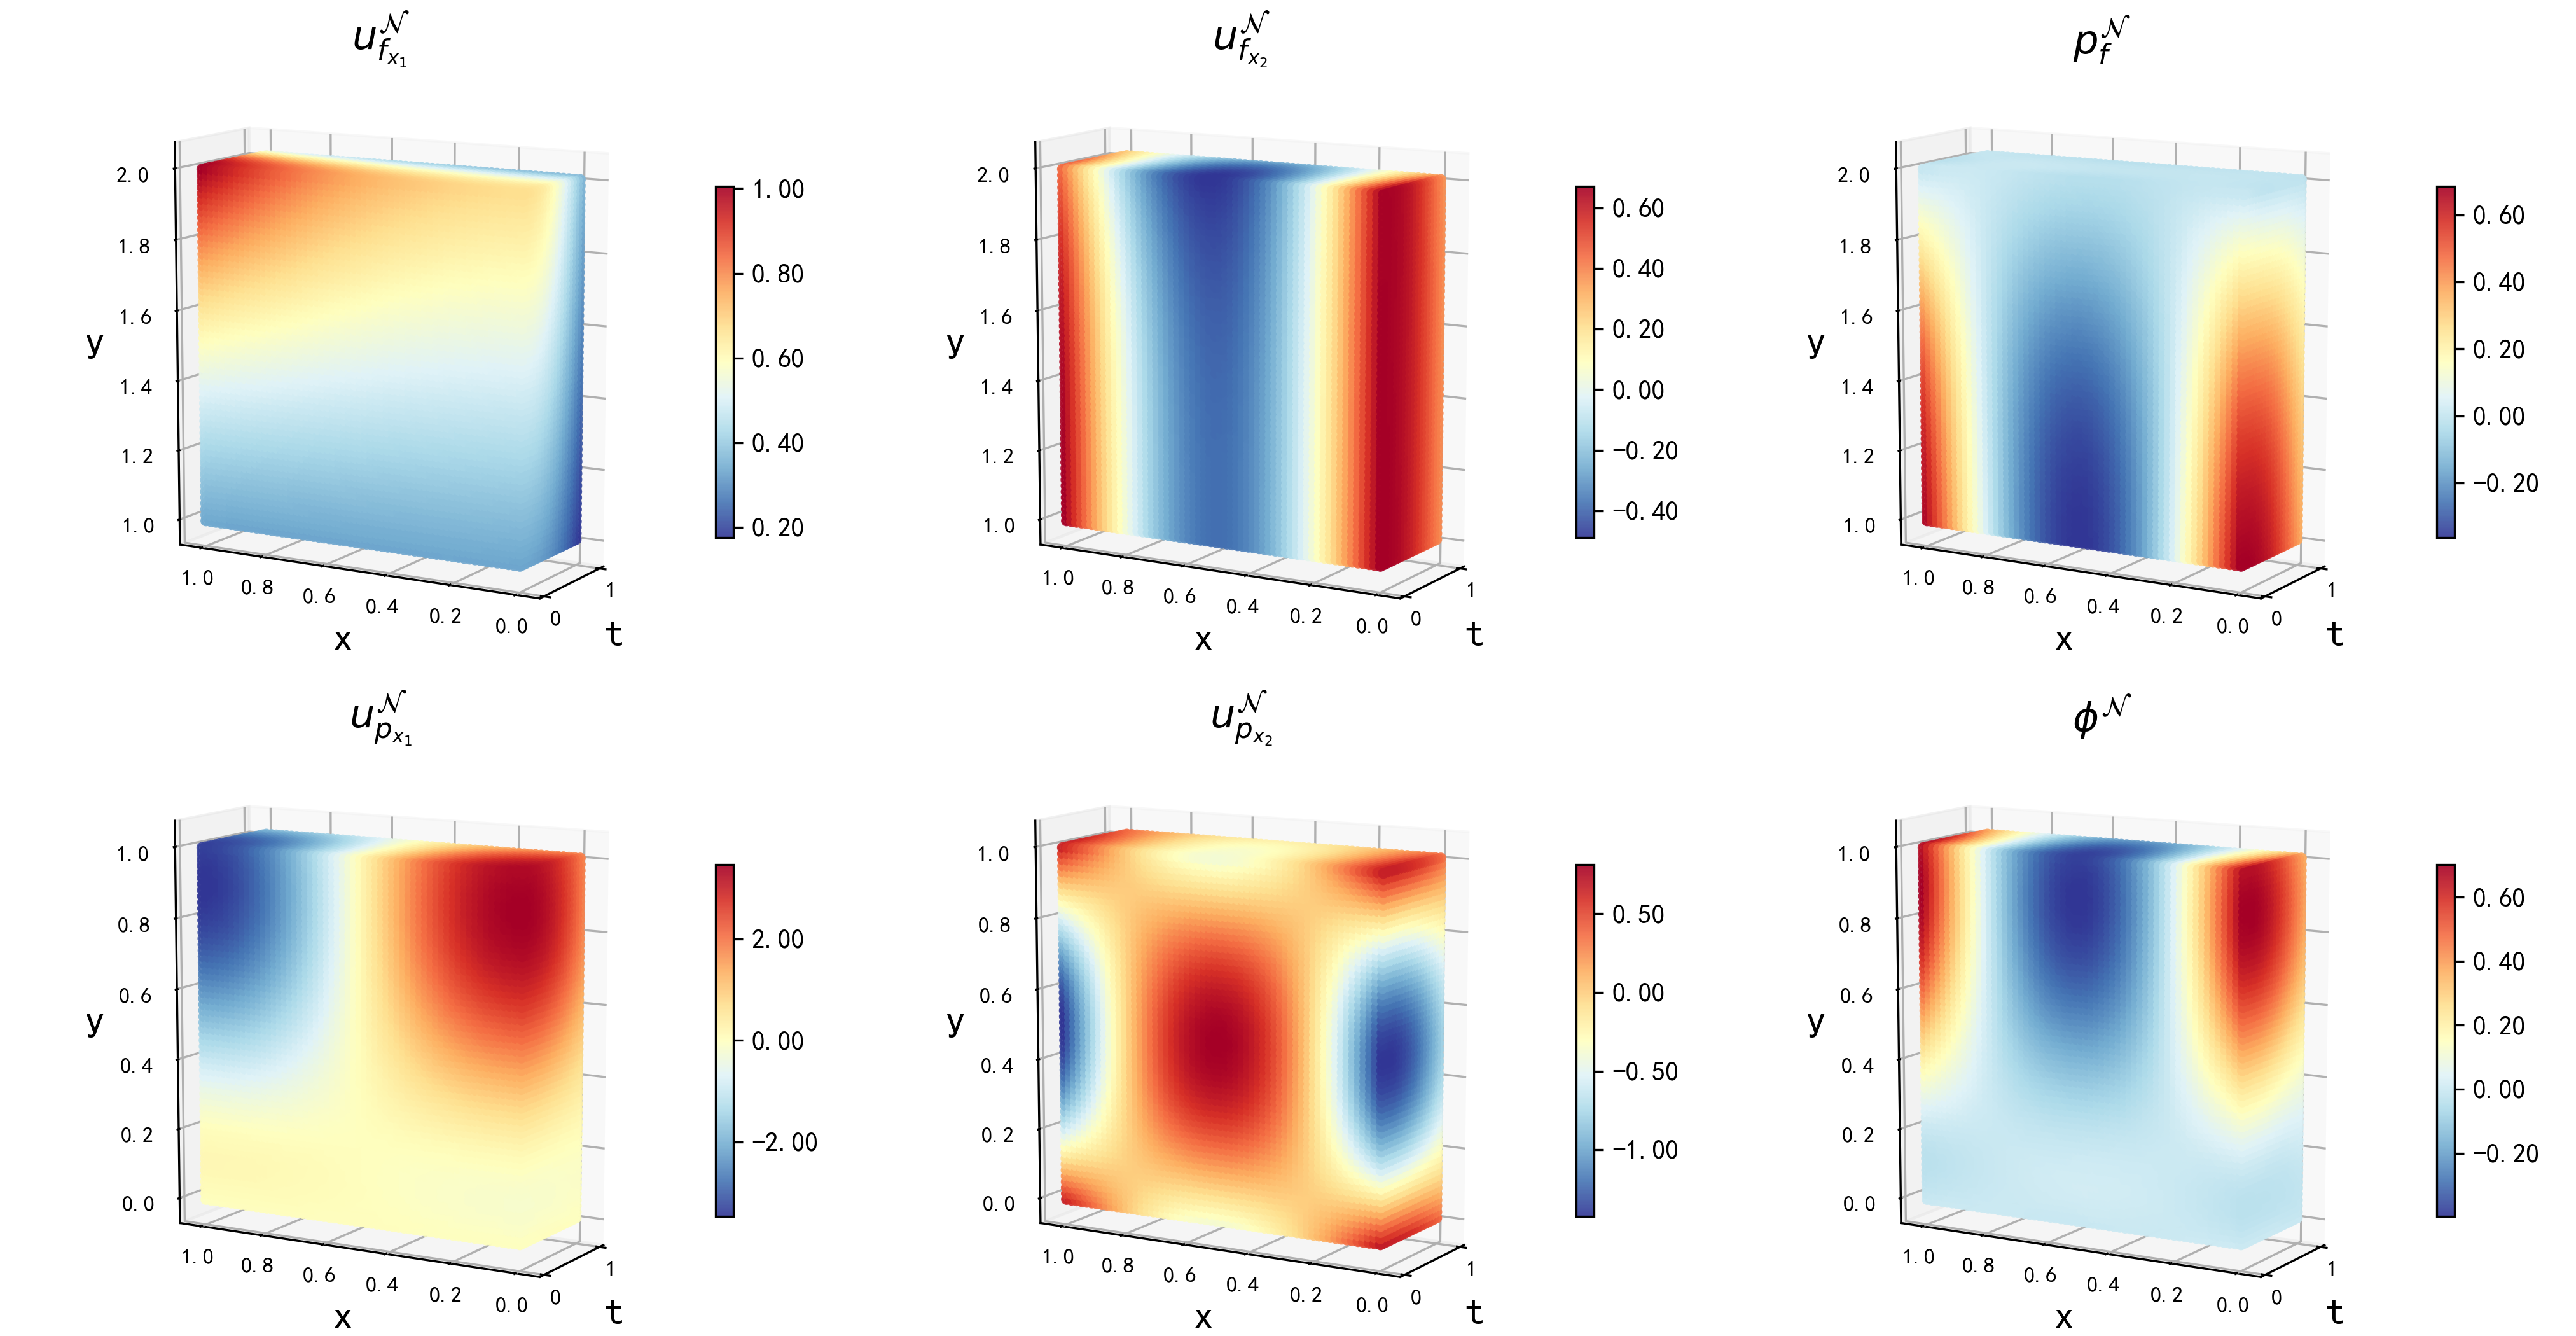
\includegraphics[width=0.75\linewidth]{images/example1_fitted.png}
    % \caption*{}
    \caption{实验一的神经网络拟合结果}
    \label{fig:example1_fitted}
\end{figure}


\section{实验二:带参数的数值实验}

本节使用另一个带有参数 $\kappa$ 的解析解测试本算法神经网络的拟合能力。这里参数 $\kappa$ 同时也影响了物理方程参数中的 $\matfmt{K} = \frac{\rho g \kappa \matfmt{I} }{\mu}$,在下述实验中将取 1.0, 0.10, 0.010,$\gf, \fp$ 同样由真解计算得到,其余方程参数以及各物理方程区域设置与实验一相同。真解公式列出如下 :

\begin{equation}\label{eq:example2}
    \left\{
    \begin{aligned}
        \Ufi[1]^* &= (1 - 2 \* x) \* (y - 1) \* \cos(t) &\textrm{ in } \Df\\
        \Ufi[2]^* &= (x \* (x - 1) + (y - 1)^2) \* cos(t) &\textrm{ in } \Df\\
        \pf^* &= \frac{1}{\kappa} \* (x \* (1 - x) \* (y - 1) + \frac{y^3}{3} - y^2 + y) \* \cos(t) &\textrm{in} \Df\\
        \Upi[1]^* &= -(-x \* (y - 1) + (1 - x) \* (y - 1))\* cos(t) &\textrm{ in } \Dp\\
        \Upi[2]^* &= -(x \* (1 - x) + y^2 - 2 \* y + 1) \* cos(t) &\textrm{ in } \Dp\\
        \pp^* &= \frac{1}{\kappa} \* (x \* (1 - x) \* (y - 1) + \frac{y^3}{3} - y^2 + y) \* \cos(t) &\textrm{in} \Dp
    \end{aligned}
    \right.
\end{equation}

网络结构采取实验一中隐藏层数为4,激活函数为 $\htf$ 的设置,此外本实验的训练策略,各训练集的采集策略均与实验一相同。在实验中发现当 $\kappa = 0.10, 0.010$ 时由于压力数值解的范围的扩大会导致网络训练的收敛速度受到影响,为此在训练中针对网络输出中代表两区域压力值的分量相应地乘上了调整系数 $10.0,100.0$ 以帮助收敛。最后实验结果由 \ref{tab:example2} 给出:

\begin{table}[H]
    \centering
    \caption{实验二结果}
    \begin{tabular}{cccc}
        \toprule
        $\kappa$ & $\relaErr_{u}$ & $\relaErr_{p}$ \\
        \midrule
        1.0        & $\num{4.1811}{-3}$ & $\num{1.0159}{-2}$ \\
        $\num{1}{-1}$ & $\num{5.2204}{-3}$ & $\num{1.5440}{-2}$ \\
        $\num{1}{-2}$ & $\num{8.7052}{-3}$ & $\num{3.9801}{-2}$ \\
        $\num{1}{-3}$ & $\num{9.9511}{-3}$ & $\num{4.3519}{-2}$ \\
        $\num{1}{-6}$ & $\num{7.5172}{-2}$ & $\num{6.1193}{-2}$ \\
        \bottomrule
    \end{tabular}
    \label{tab:example2}
\end{table}

以参数 $\kappa = 0.1$ 为例,其真解与拟合结果如图 \ref{fig:example2_exact},\ref{fig:example2_fitted} 所示,

\begin{figure}[H]
    \centering
    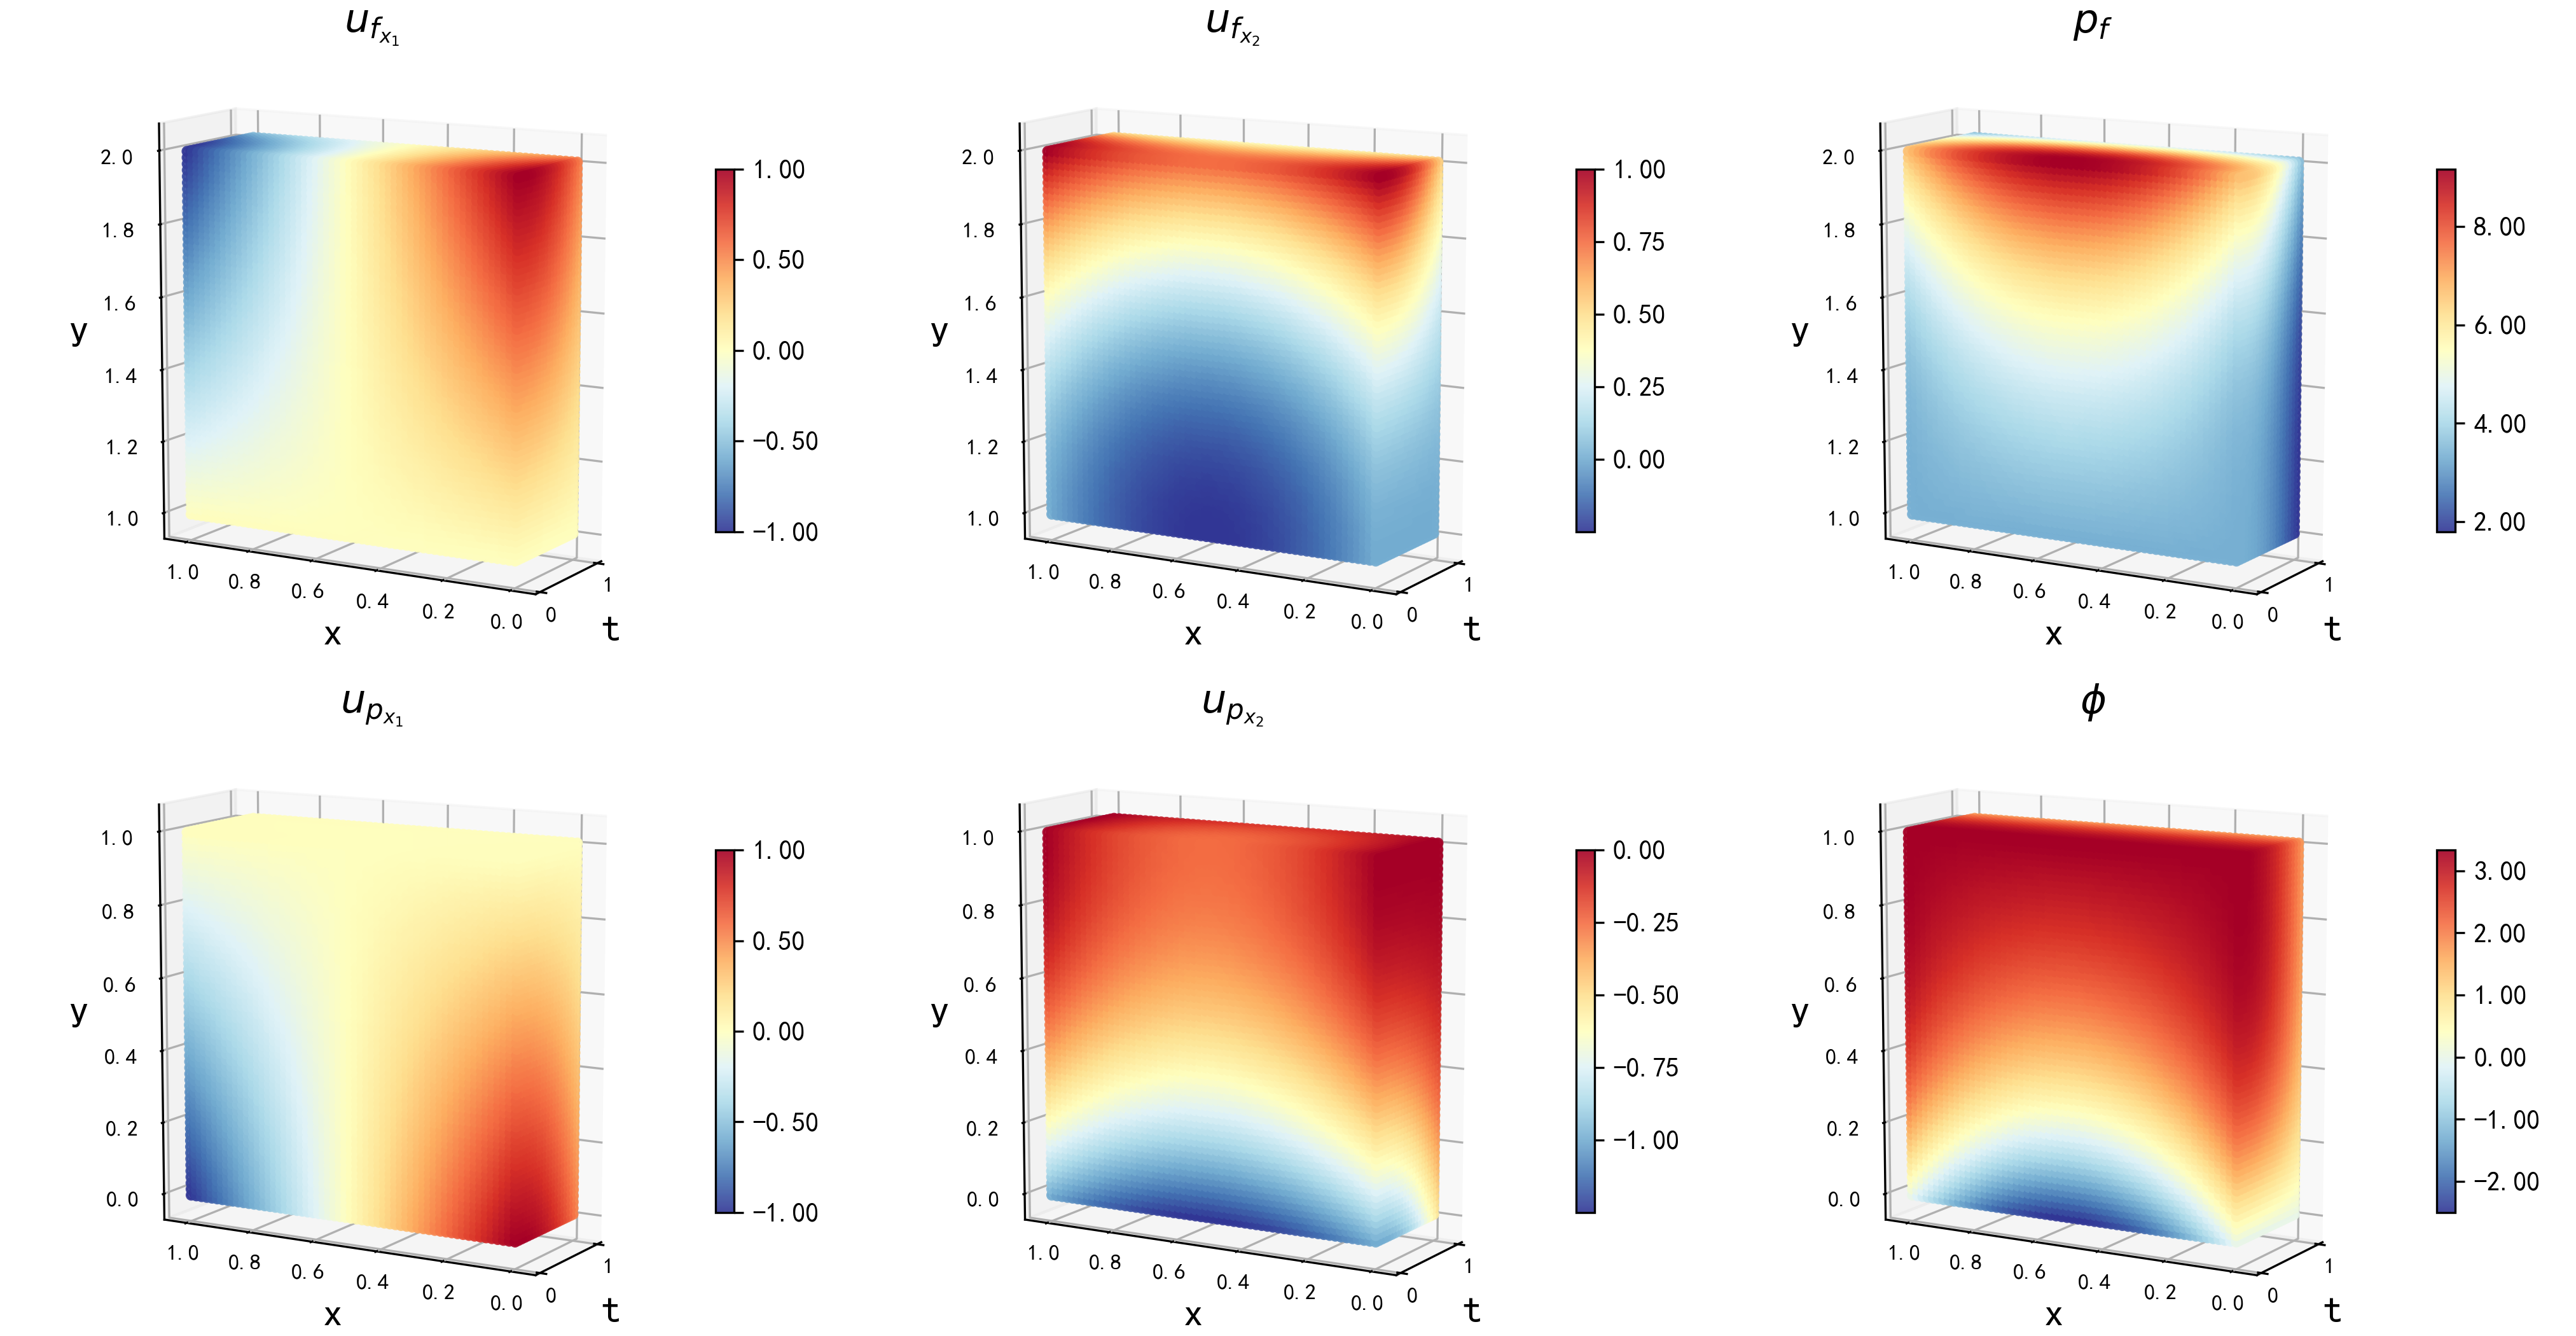
\includegraphics[width=0.75\linewidth]{images/example2_exact.png}
    % \caption*{}
    \caption{实验二的数值真解}
    \label{fig:example2_exact}
    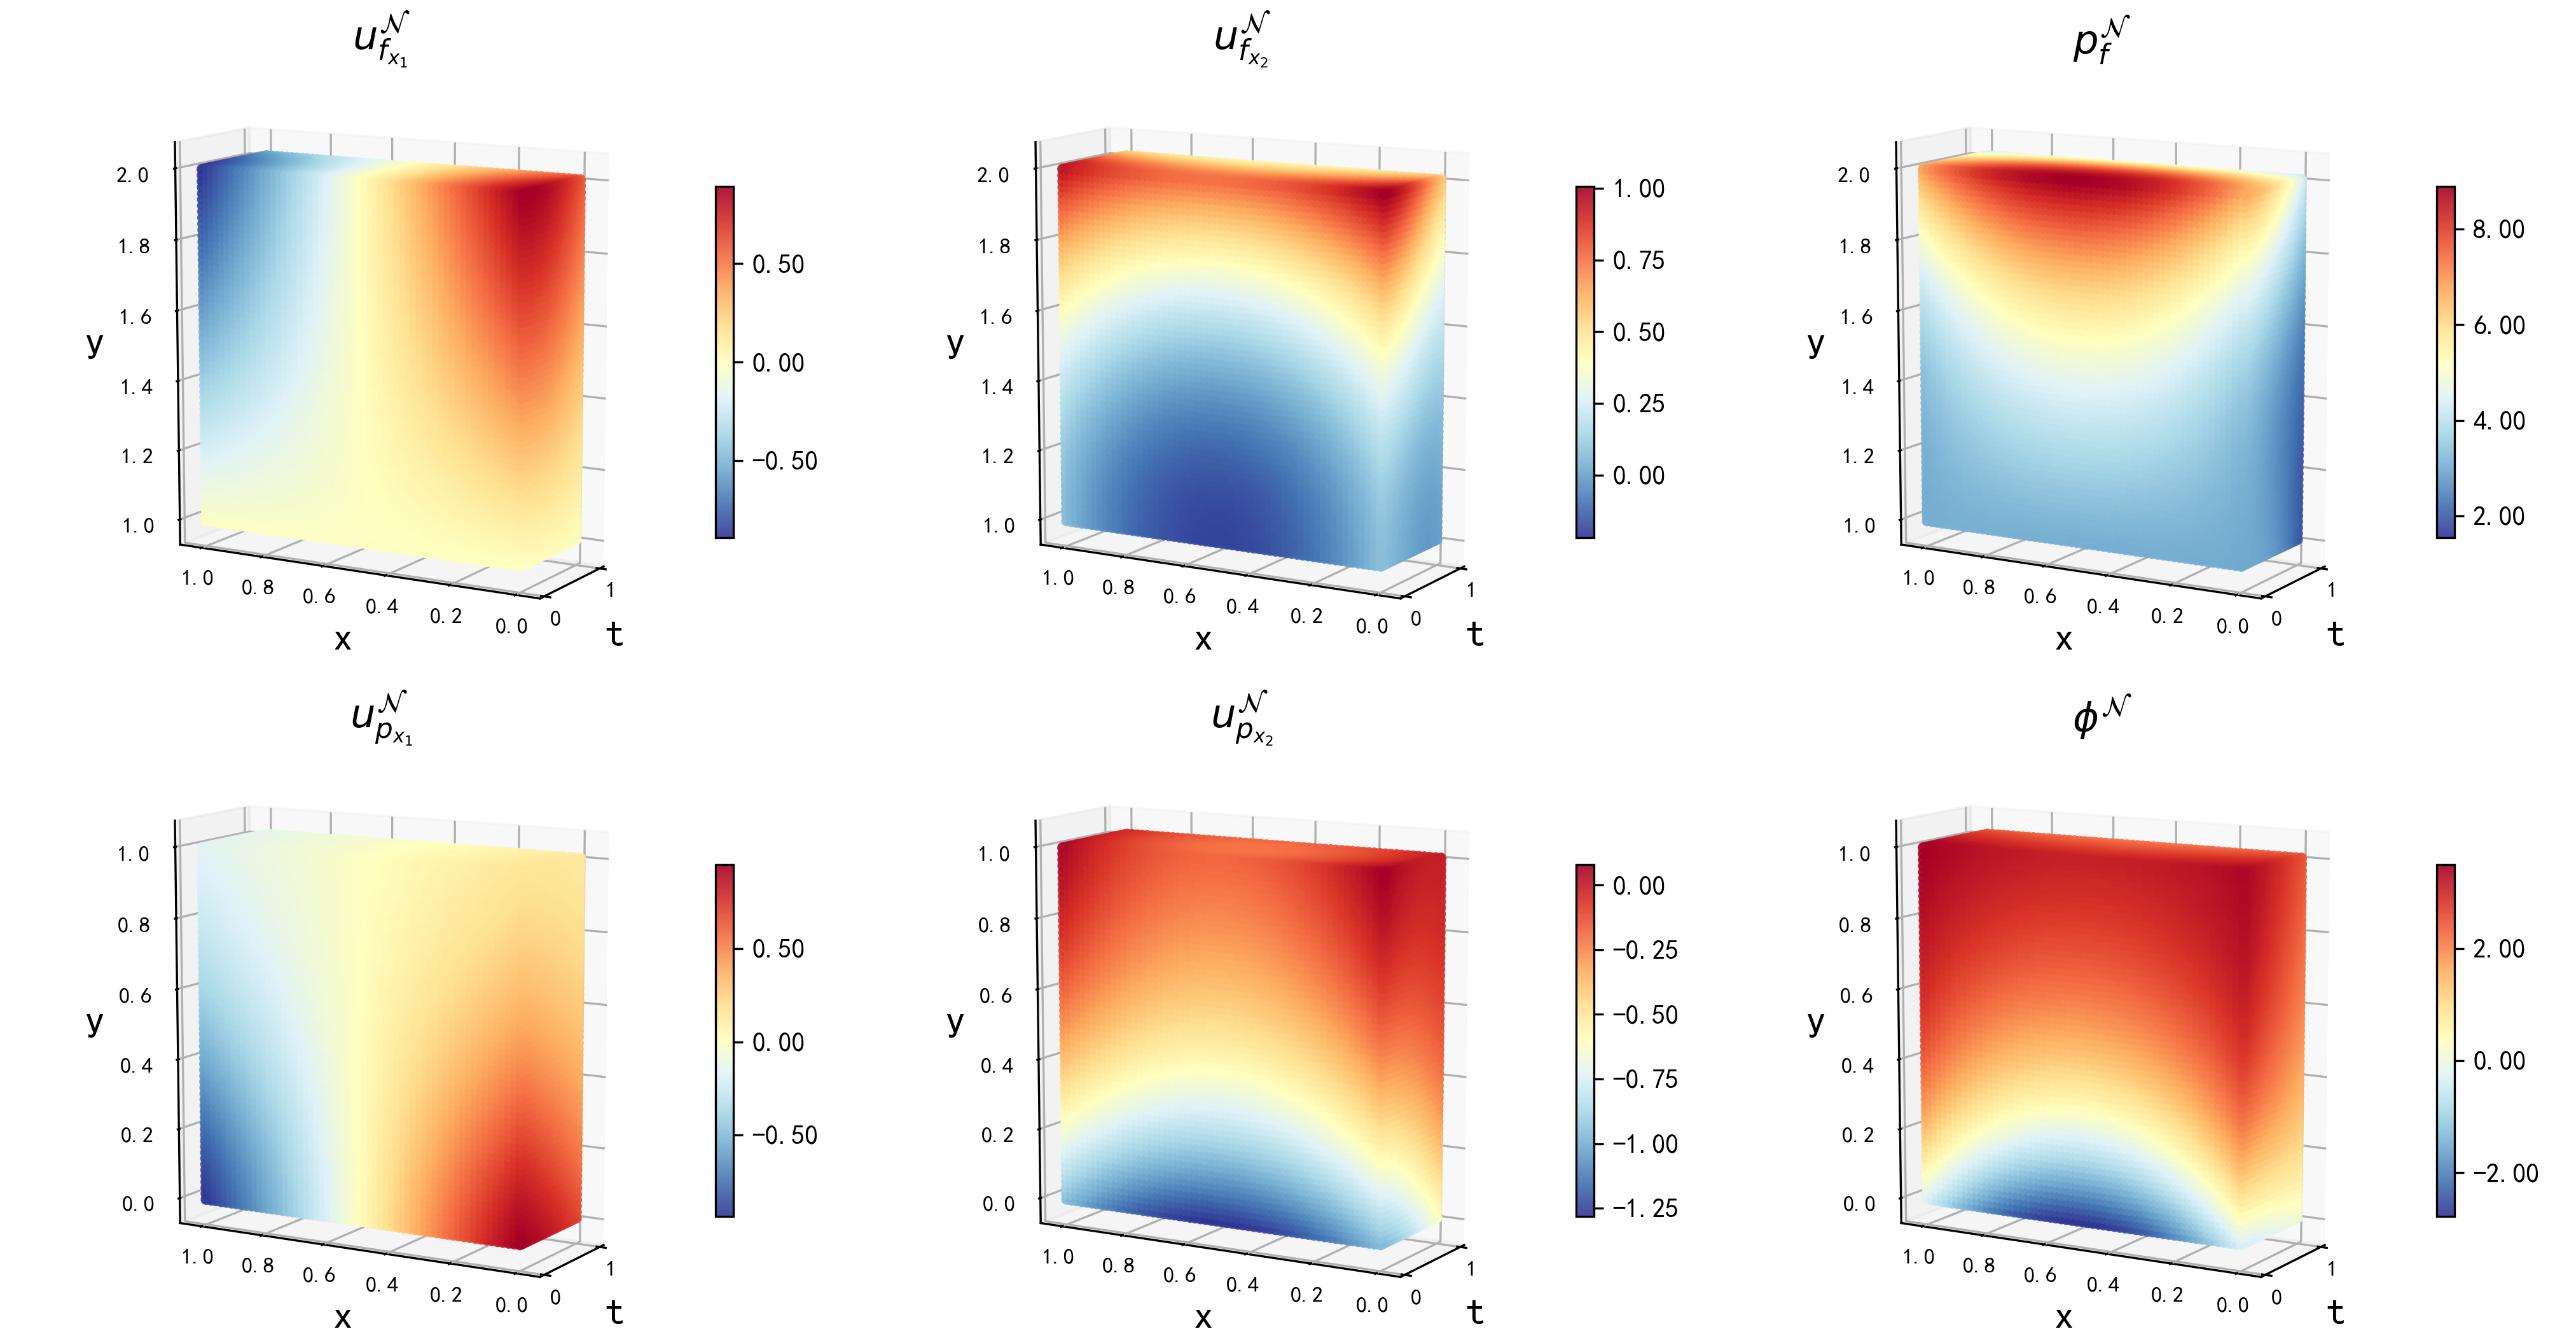
\includegraphics[width=0.75\linewidth]{images/example2_fitted.png}
    % \caption*{}
    \caption{实验二的神经网络拟合结果}
    \label{fig:example2_fitted}
\end{figure}

\section{实验三:稳态实验}
本节针对稳态形式的 Navier-Stokes/Darcy 耦合模型进行求解。所谓稳态形式,即去掉了物理方程中的时间项,同时需要去掉各物理区域的初值条件。此时物理模型描述的是一类状态稳定的流体运动,该耦合模型方程如 ~\eqref{eq:Stable} 所示:

\begin{equation}\label{eq:Stable}
    \left\{
        \begin{aligned}
            \rho (\Uf \cdot \gradOp) \Uf - \gradOp \cdot \opTf &= \rho\gf & & \textrm{ in } \Of\\  
            \gradOp \cdot \Uf &= 0 & & \text{ in } \Of \\
            \Uf &= \Uf^{\Bf} & & \text{ on } \Bf,\\
            \gradOp \cdot \Up &=\fp & & \text { in } \Op, \\
            \Up &= -\matfmt{K} \gradOp \pp & & \text { in } \Op.\\
            \pp &=\pp_{\Bp} & & \text { on } \Bp
        \end{aligned}
    \right.
\end{equation}

注意稳态耦合模型的交界面条件保持不变,因其本就没有时间项。

第四章中两个实验的解析解都可以很容易修改为其对应的稳态形式,方程如 ~\eqref{eq:example_stable1},~\eqref{eq:example_stable2} 所示,其空间区域以及对应物理方程各参数同实验一。

\begin{equation}\label{eq:example_stable1}
    \left\{
    \begin{aligned}
        \Ufi[1]^* &= \frac{1}{3} \* (x^2 \* (y-1)^2 + y) &\textrm{ in } \Df\\
        \Ufi[2]^* &= \frac{1}{3} \* (-\frac{2}{3} \* x \* (y-1)^3 + 2 - \pi \* sin(\pi \* x)) &\textrm{ in } \Df\\
        \pf^* &= \frac{1}{3} \* (2 - \pi \* sin(\pi \* x)) \* sin(\pi \* \frac{y}{2}) &\textrm{ in } \Df\\
        \Upi[1]^* &= \frac{\pi^2}{3} \* (-y - cos(\pi \* y) + 1) \* cos(\pi \* x) &\textrm{ in } \Dp\\
        \Upi[2]^* &= \frac{1}{3} \* \left(\pi \* sin(\pi \* x) - 2\right) \* \left(\pi \* sin(\pi \* y) - 1 \right) &\textrm{ in } \Dp\\
        \pp^* &= \frac{1}{3} \* (2 - \pi \* sin(\pi \* x)) \* (1 - y - cos(\pi \* y)) &\textrm{ in } \Dp
    \end{aligned}
    \right.
\end{equation}

\begin{equation}\label{eq:example_stable2}
    \left\{
    \begin{aligned}
        \Ufi[1]^* &= (1 - 2 \* x) \* (y - 1) &\textrm{ in } \Df\\
        \Ufi[2]^* &= (x \* (x - 1) + (y - 1)^2) &\textrm{ in } \Df\\
        \pf^* &= \frac{1}{\kappa} \* (x \* (1 - x) \* (y - 1) + \frac{y^3}{3} - y^2 + y) &\textrm{ in } \Df\\
        \Upi[1]^* &= -(-x \* (y - 1) + (1 - x) \* (y - 1)) &\textrm{ in } \Dp\\
        \Upi[2]^* &= -(x \* (1 - x) + y^2 - 2 \* y + 1) &\textrm{ in } \Dp\\
        \pp^* &= \frac{1}{\kappa} \* (x \* (1 - x) \* (y - 1) + \frac{y^3}{3} - y^2 + y) &\textrm{ in } \Dp
    \end{aligned}
    \right.
\end{equation}

容易验证两个解析解均满足上述公式 ~\eqref{eq:Stable} 以及原交界面条件 ~\eqref{eq:Interface} 。

要使本文提出的神经网络求解算法拟合上述真解,只需相应构造出方程 ~\eqref{eq:Stable} 对应的损失函数进行替换,构造方法与第二章所描述的完全相同,同时删除初值条件的损失即可,最后得到公式 ~\eqref{eq:stable_lossf}~\eqref{eq:stable_lossp}:


\begin{equation}\label{eq:stable_lossf}
    \begin{aligned}
        &\Lossf \\
        &= \toLoss{\TDf}{\x,\gf(\x)}{d}{
            \rho (\NUf \cdot \gradOp) \NUfi 
                - \compx{(\gradOp \cdot \opT{\NUf}{\Npf{\cdot}})} - \rho \compx{\gf}
        } \\
        &+
        \toscaLoss{\TDf}{\x}{
            (\gradOp \cdot \NUf)(\x) - 0
        } \\
        &+
        \toLoss{\TBDf}{\x,\Uf^{\Bf}(\x)}{d}{
            \NUfi(\x) - \compx{u^{\Bf}_{f}}
        }
    \end{aligned}
\end{equation}
\begin{equation}\label{eq:stable_lossp}
    \begin{aligned}
        &\Lossp \\ 
        &= \toscaLoss{\TDp}{\x,\fp(\x)}{
            (\gradOp \cdot \NUp)(\x) - \fp(\x)
        } \\
        &+
        \toLoss{\TDp}{\x}{d}{
            \NUpi(\x) + \compx{(\matfmt{K} \gradOp \Npp)}
        } \\
        &+
        \toscaLoss{\TBDp}{\x,{\pp_{\Bp}}(\x)}{
            \Npp(\x) - \pp_{\Bp}(\x)
        }
    \end{aligned}
\end{equation}

实验的网络结构、训练策略以及各训练集的采集策略均与实验二相同(数据采集比例相对不变),实验结果见表 \ref{tab:example_stable}。

\begin{table}[htb]
    \centering
    \caption{稳态实验结果}
    \begin{tabular}{cccc}
        \toprule
        真解公式 & $\relaErr_{u}$ & $\relaErr_{p}$ \\
        \midrule
        公式 ~\eqref{eq:example_stable1}  & $\num{2.7499}{-2}$ & $\num{6.9892}{-2}$ \\
        公式 ~\eqref{eq:example_stable2},$\kappa = 1.0$   & $\num{7.0199}{-3}$ & $\num{2.8815}{-2}$ \\
        公式 ~\eqref{eq:example_stable2},$\kappa = \num{1}{-1}$  & $\num{7.0020}{-3}$ & $\num{2.5232}{-2}$ \\
        公式 ~\eqref{eq:example_stable2},$\kappa = \num{1}{-2}$ & $\num{9.6692}{-3}$ & $\num{4.7237}{-2}$ \\
        公式 ~\eqref{eq:example_stable2},$\kappa = \num{1}{-3}$ & $\num{1.1323}{-2}$ & $\num{7.5991}{-2}$ \\
        \bottomrule
    \end{tabular}
    \label{tab:example_stable}
\end{table}

图 \ref{fig:example_stable1} \ref{fig:example_stable2} 展示了部分真解与拟合结果的直观对比情况。虽然稳态实验中网络的训练无需考虑时间项,但同时已知条件也缺少了初值信息,因此网络拟合难度也不亚于非稳态实验。从结果可以看出算法求解依然是成功的。

\begin{figure}[H]
    \centering
    \subcaptionbox{ 数值真解 \label{fig:example_stable1_exact}}{
        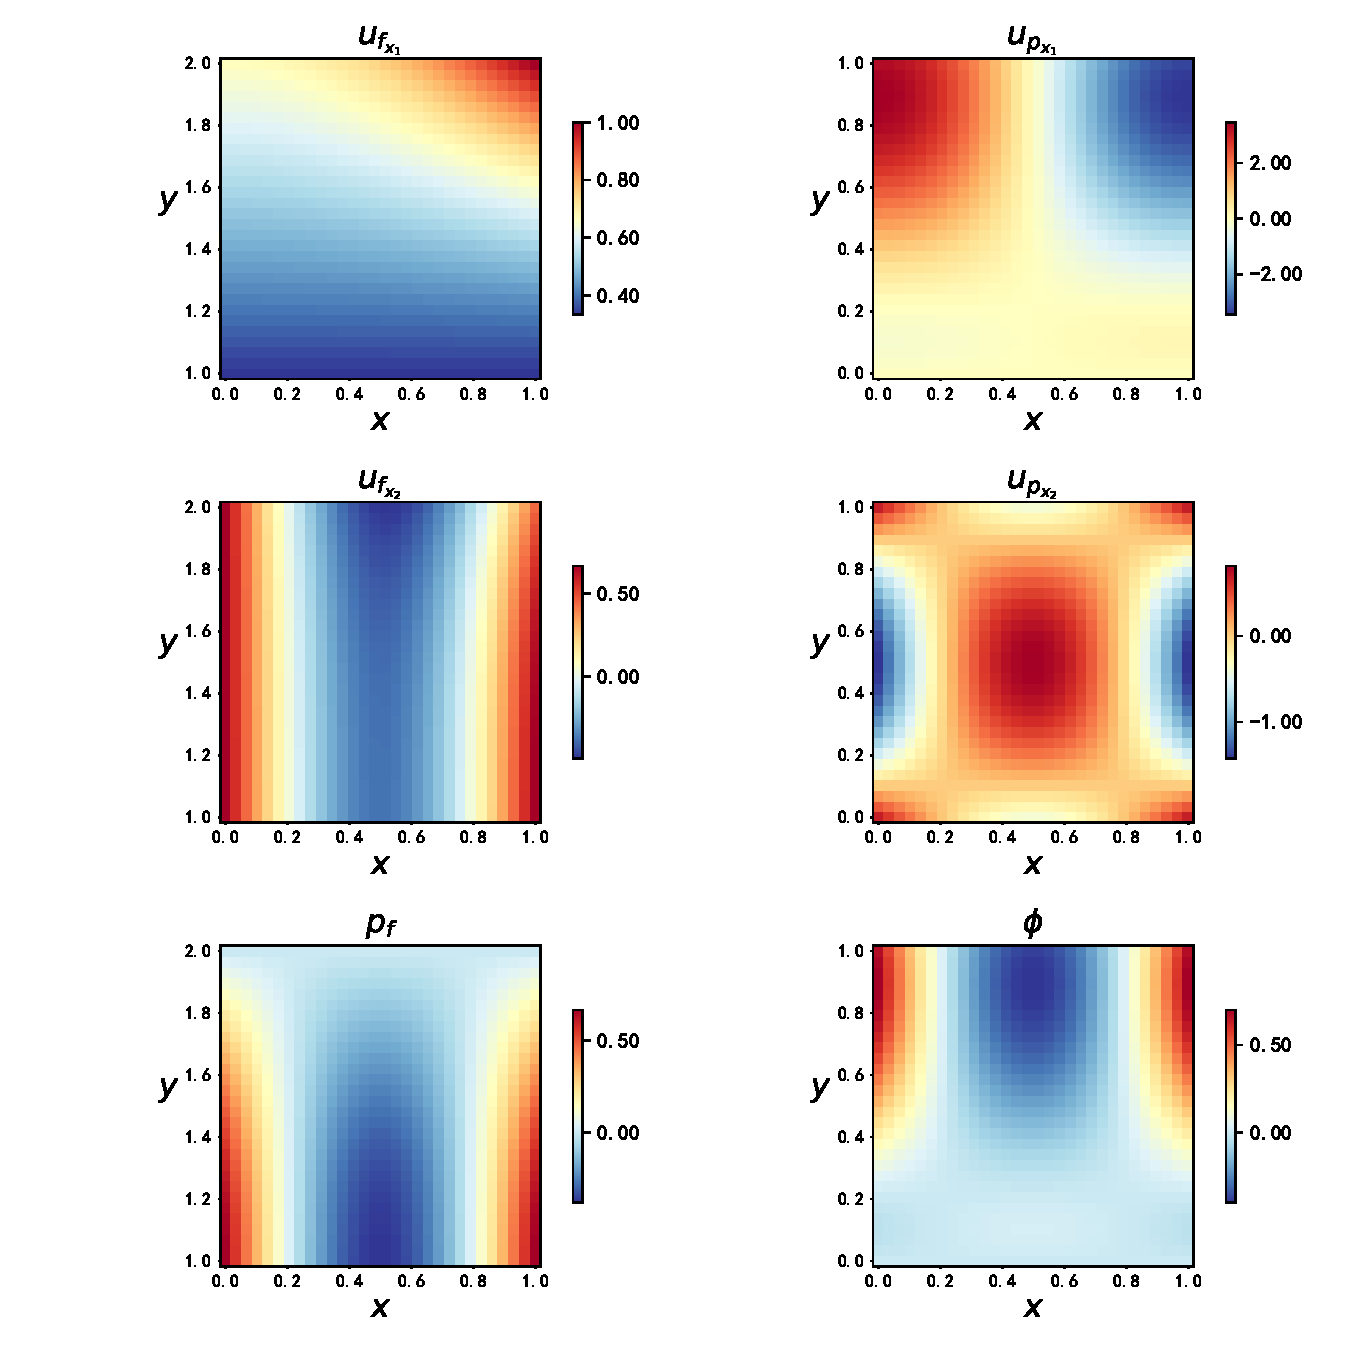
\includegraphics[width=0.45\linewidth]{images/example_stable1_exact.pdf}
    }\subcaptionbox{ 神经网络拟合结果 \label{fig:example_stable1_fitted}}{
        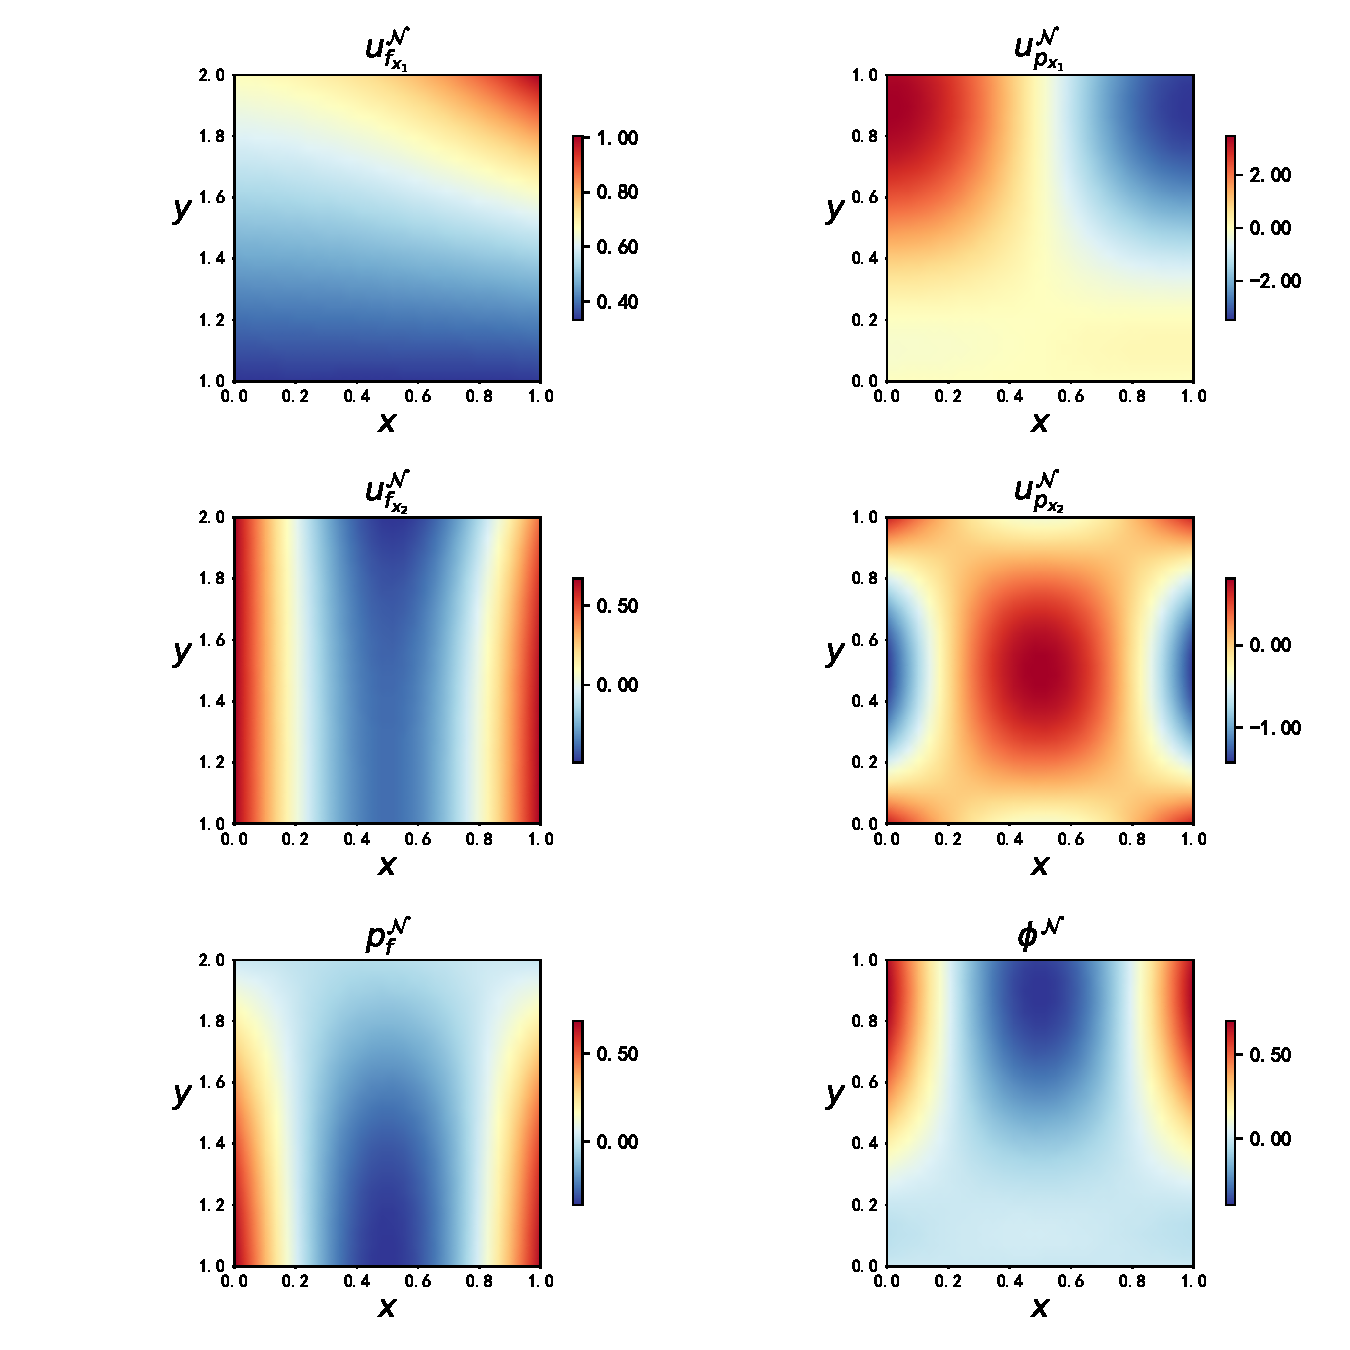
\includegraphics[width=0.45\linewidth]{images/example_stable1_fitted.pdf}
    }
    \caption{ 公式 ~\eqref{eq:example_stable1} 的真解与拟合结果对比图}
    \label{fig:example_stable1}
    \subcaptionbox{ 数值真解 \label{fig:example_stable2_exact}}{
        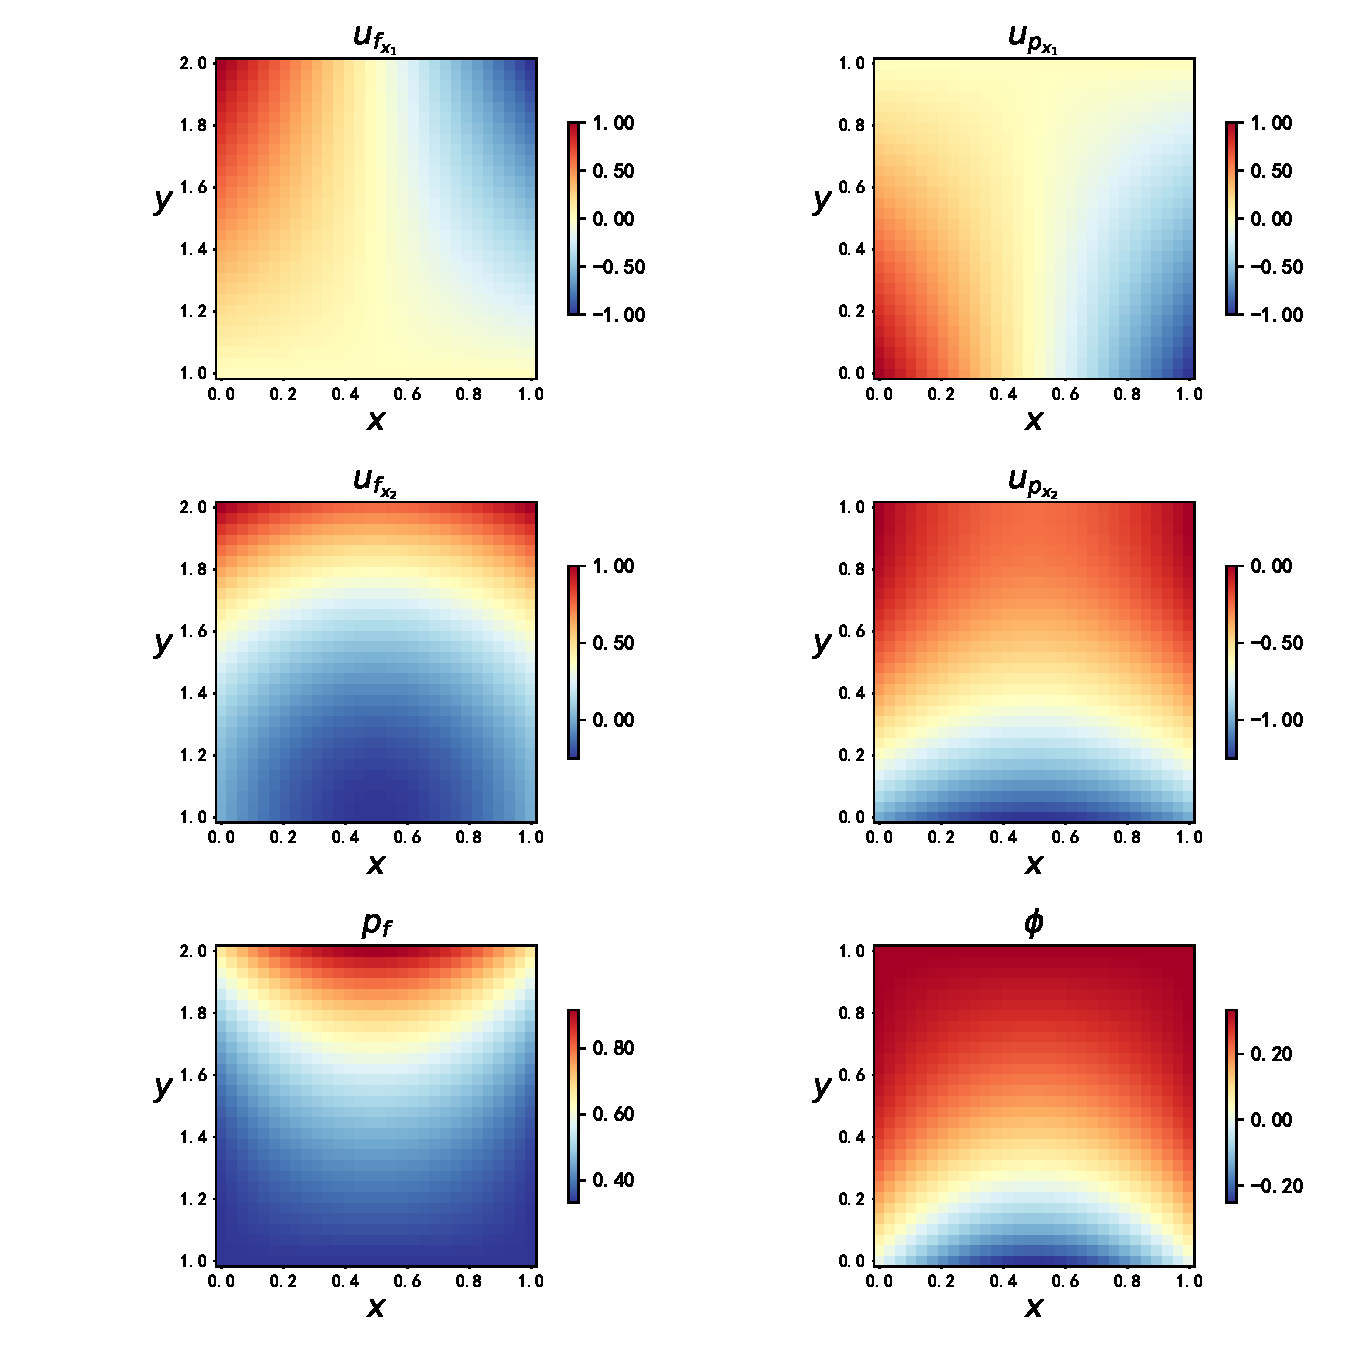
\includegraphics[width=0.45\linewidth]{images/example_stable2_exact.pdf}
    }\subcaptionbox{ 神经网络拟合结果 \label{fig:example_stable2_fitted}}{
        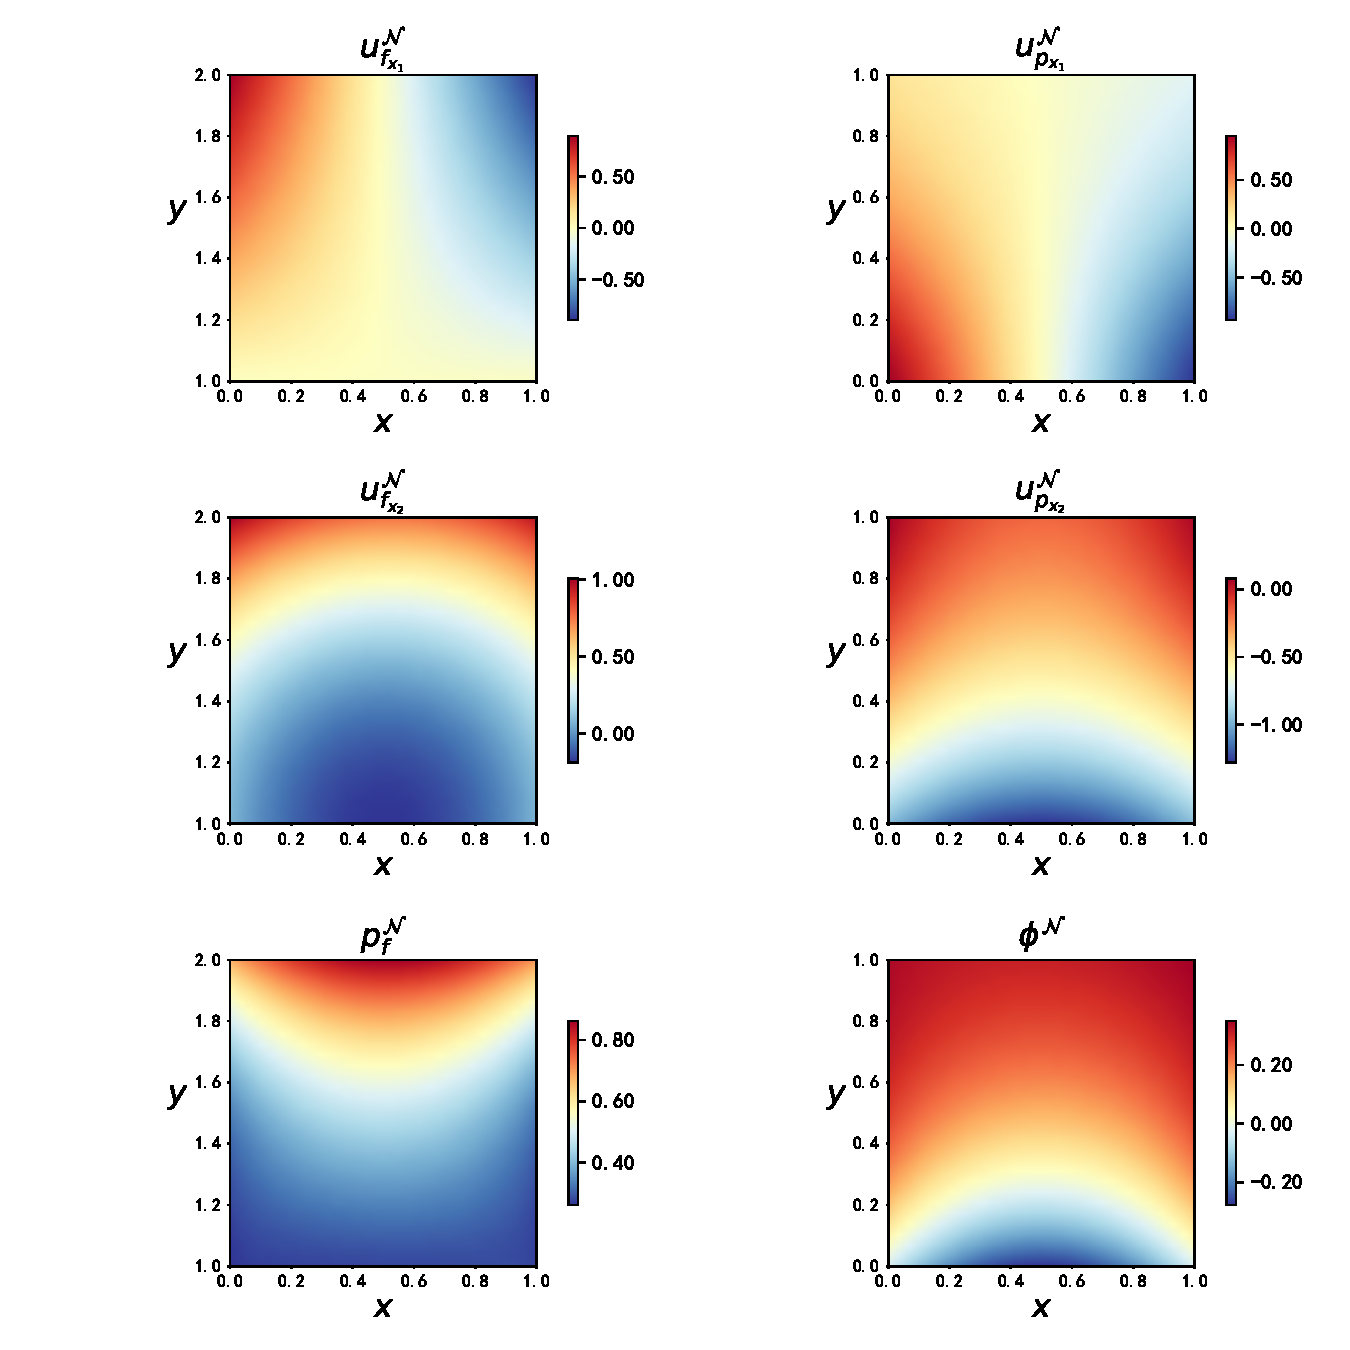
\includegraphics[width=0.45\linewidth]{images/example_stable2_fitted.pdf}
    }
    \caption{ 公式 ~\eqref{eq:example_stable2} 的真解与拟合结果对比图}
    \label{fig:example_stable2}
\end{figure}

\section{实验四:BJS 交界面实验}

关于 Navier-Stokes/Darcy 耦合模型的BJ交界面条件,存在一种公认的简化形式, 在实践中观察到多孔介质流区域中 $\Up \cdot \tau_i$ 这一项的大小要远远小于其他项,因此是可以被忽略的。这就形成了著名的 BJS(Beavers-Joseph-Saffman)交界面条件 \cite{saffman1971boundary}:

\begin{equation}\label{eq:BJS}
    \begin{aligned}
        -\left(\opTf \vec{n} \right) \cdot \vec{\tau}_i = \alpha \sqrt{\frac{g \rho \mu}{(\matfmt{K} \vec{\tau}_i) \cdot \vec{\tau}_i}} \Uf \cdot \vec{\tau}_i, i=1,\cdots,(d-1) \quad \text{ on } \iB
    \end{aligned}
\end{equation}

本算例将对采用如上交界面条件的耦合模型进行求解,其对应的解析解如下,容易验证其满足公式 ~\eqref{eq:NS},~\eqref{eq:Darcy} 与 ~\eqref{eq:BJS}:

\begin{equation}\label{eq:example_BJS}
    \left\{
    \begin{aligned}
        \Ufi[1]^* &= -\sin(\pi \* y) \* \cos(t) \* cos(\pi \* x) &\textrm{ in } \Df\\
        \Ufi[2]^* &= \sin(\pi \* x) \* \cos(t) \* \cos(\pi \* y) &\textrm{ in } \Df\\
        \pf^* &= \sin(\pi \* x) \* \cos(t) &\textrm{ in } \Df\\
        \Upi[1]^* &= -\pi \* y \* \cos(t) \* \cos(\pi \* x) &\textrm{ in } \Dp\\
        \Upi[2]^* &= - \sin(\pi \* x) \* \cos(t) &\textrm{ in } \Dp\\
        \pp^* &= y \* \sin(\pi \* x) \* \cos(t) &\textrm{ in } \Dp
    \end{aligned}
    \right.
\end{equation}

类似于上一节的稳态实验,将 cPINNs 迁移到此耦合模型只需要将求解算法中 BJ 交界面条件对应的损失函数替换为 BJS 交界面条件即可,这里 BJS 交界面条件的损失函数如下:

\begin{equation}
    \begin{aligned}
        &\Lossi_{3} \\
        &= \sum_{i=1}^{d-1} 
            \toscaLossPre{\TiBD}{\x}
            \left|
                -(\left(\opT{\NUf}{\Npf} \vec{n} \right) \cdot \vec{\tau}_i)(\x)
            \right.\\
            &\hspace*{8em} \left. - \alpha \sqrt{\frac{g \rho \mu}{(\matfmt{K} \vec{\tau}_i) \cdot \vec{\tau}_i}} (\NUf \cdot \vec{\tau}_i)(\x)
            \right|^{p}
    \end{aligned}
\end{equation}

其余的网络结构等配置也与实验三相同,实验结果如 \ref{tab:example_BJS} 所示,算法依然能够拟合出数值解:

\begin{table}[H]
    \centering
    \caption{稳态实验结果}
    \begin{tabular}{cccc}
        \toprule
        真解公式 & $\relaErr_{u}$ & $\relaErr_{p}$ \\
        \midrule
        公式 ~\eqref{eq:example_BJS}  & $\num{4.3153}{-3}$ & $\num{8.7145}{-3}$ \\
        \bottomrule
    \end{tabular}
    \label{tab:example_BJS}
\end{table}

真解与拟合结果对比图如 \ref{fig:example_BJS_exact},\ref{fig:example_BJS_fitted} 所示,可以看出各物理量的数值分布几乎相同:

\begin{figure}[H]
    \centering
    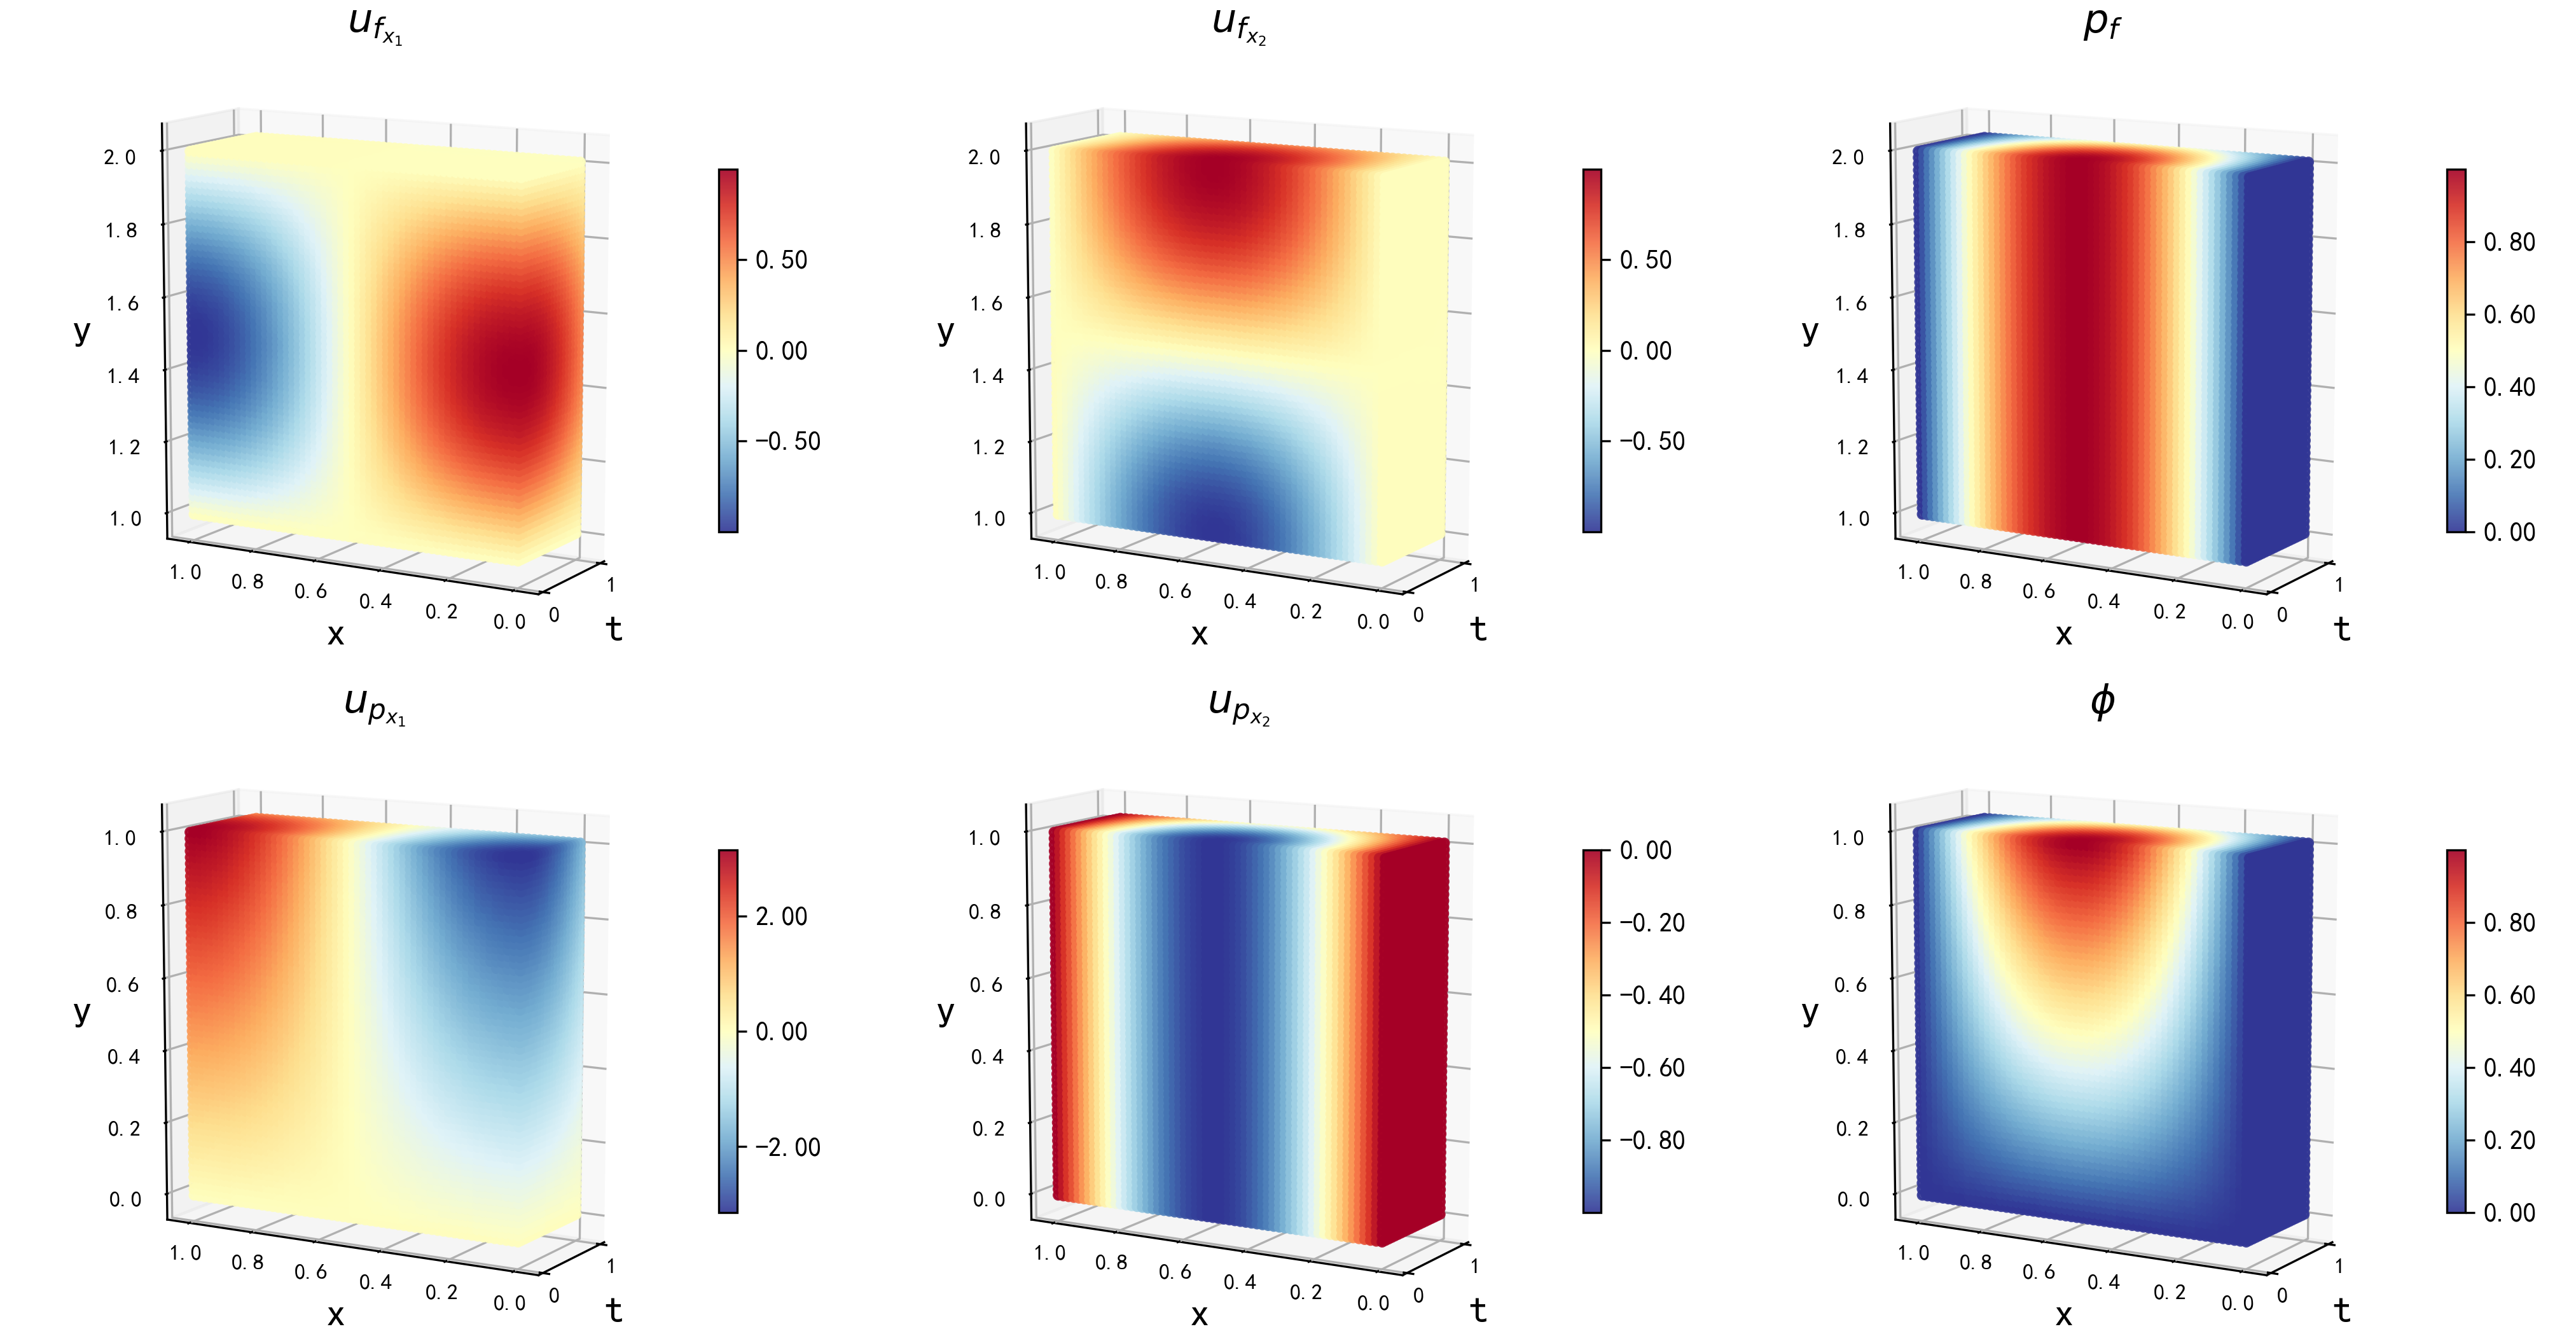
\includegraphics[width=0.75\linewidth]{images/example_BJS_exact.png}
    % \caption*{}
    \caption{BJS实验公式 ~\eqref{eq:example_BJS} 的数值真解}
    \label{fig:example_BJS_exact}
    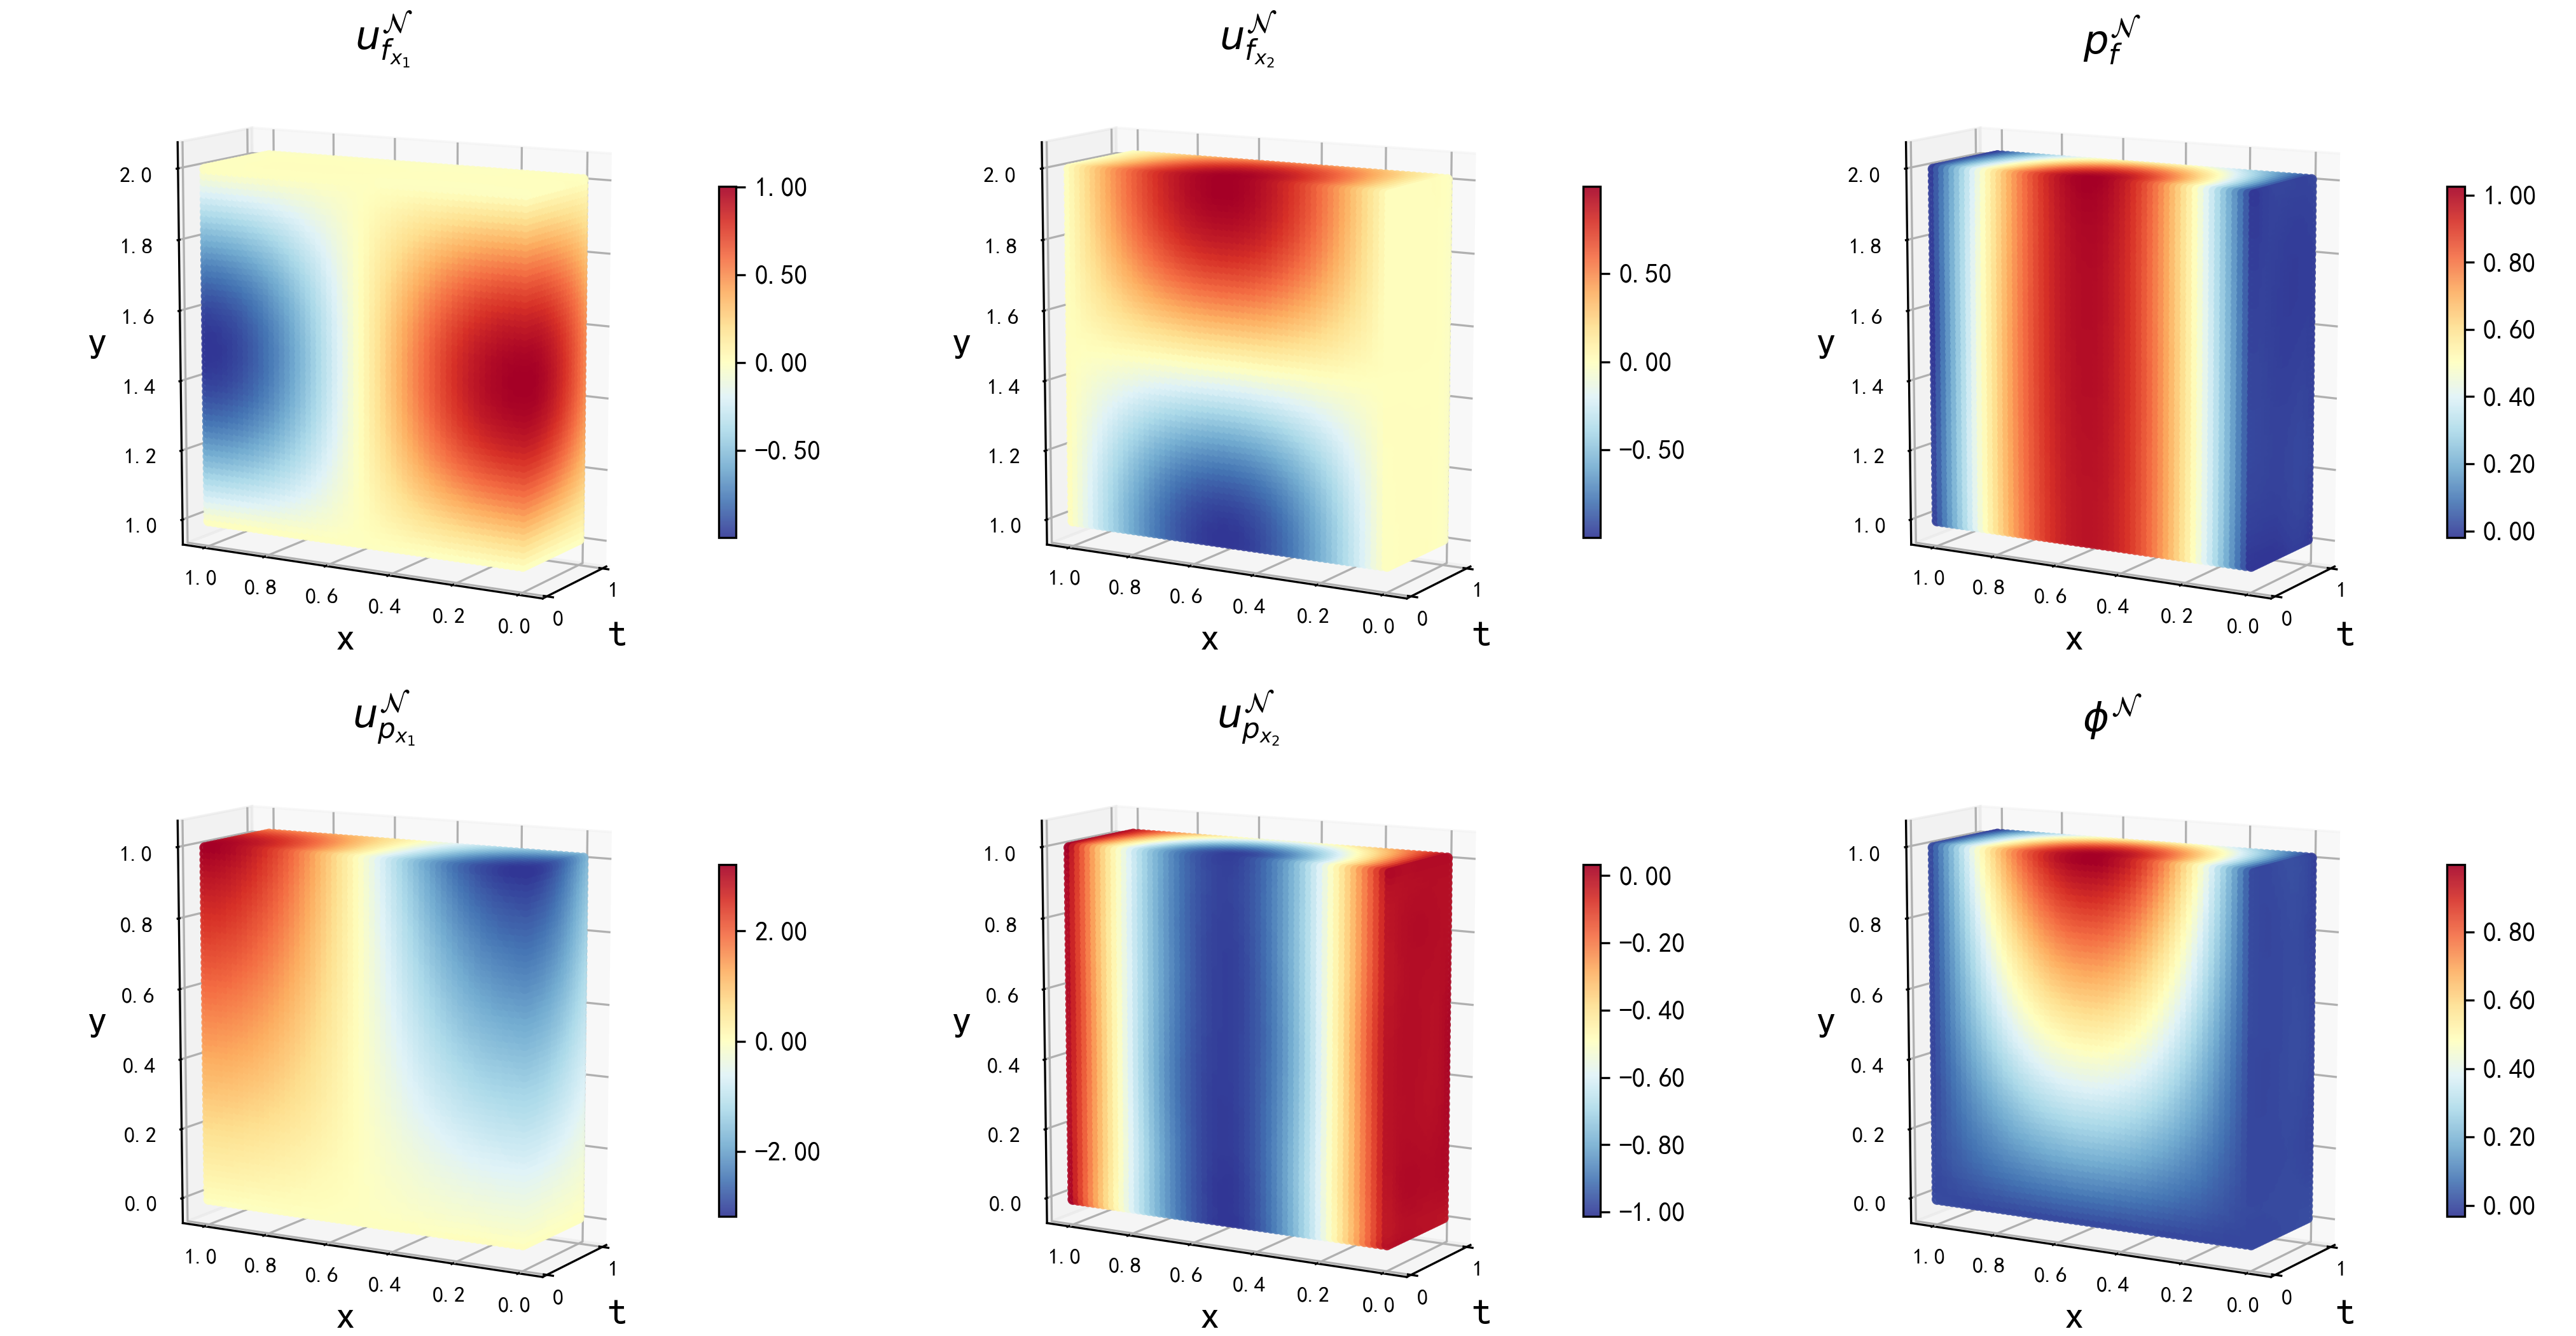
\includegraphics[width=0.75\linewidth]{images/example_BJS_fitted.png}
    % \caption*{}
    \caption{BJS实验公式 ~\eqref{eq:example_BJS} 的神经网络拟合结果}
    \label{fig:example_BJS_fitted}
\end{figure}

以上实验结果说明网络对不同的数值算例均有一定的拟合能力。


